\chapter{Signal Reconstruction on Cartesian Product Graphs}

\label{chap:gsr_2d}

\lhead{Chapter 3. \emph{Regression and Reconstruction on Cartesian Product Graphs}}

% What are we doing? 

In this chapter, we address the topic of signal reconstruction over general two-dimensional Cartesian product graphs, where an arbitrary set of signal elements is missing. The first key objective is to present a novel Bayesian model for this purpose, based on our formulation of multivariate graph filters, where a smooth underlying signal must be inferred given a noisy partial observation. The second is to produce two scalable iterative algorithms for computing the posterior mean and investigate their respective convergence properties both theoretically and empirically. 

% why is this useful?

As discussed in \cref{sec:GSR_review}, Graph Signal Reconstruction (GSR) is a topic that has received substantial attention in the last decade. Whilst the majority of past models have focused on the reconstruction of a single one-dimensional signal, with some recent models extending this to time-varying signals, our approach can be seen as a natural generalisation that encompasses two-dimensional matrix signals with arbitrary undirected graphs underlying each axis. Furthermore, we believe our Bayesian approach can offer new insight into multivariate correlation structure over irregular topologies. Since efficient computation is a critical factor in real-world applications of GSR, we devote substantial attention to a careful analysis of computational complexity. In doing so, we show how the two iterative algorithms we present possess different convergence behaviour and implementation details, making the optimal choice dependent on the hyperparameters, data composition, and graph sparsity. 


% chapter layout

We begin in \cref{sec:reg_and_rec_intro} by reviewing the concept of a graph product, explaining our rationale for focusing on the Cartesian product in particular, and introducing our model for two-dimensional anisotropic filters. In \cref{sec:gsr_cpg}, we present our statistical model for graph signal reconstruction on a Cartesian product graph and derive the two algorithms for solving the posterior mean. These encompass a Stationary Iterative Method (SIM) based on matrix splitting and a Conjugate Gradient Method (CGM) using a graph-spectral preconditioner. In addition, we show how the SIM can be implemented using Chebyshev polynomials to avoid Laplacian eigendecomposition. To end this section, we demonstrate the utility of these models using a dataset comprising daily SARS-CoV-19 case rates across the UK. Finally, in \cref{sec:convergence}, we engage in an in-depth analysis of the convergence properties of each method and propose practical guidelines for method selection. 


\section{Graph Products}

\label{sec:reg_and_rec_intro}

In this chapter, we will be primarily concerned with signal processing on \textit{Cartesian product graphs}. This special class of graph finds applications in numerous areas, such as video, hyper-spectral image processing and network time series problems. However, the Cartesian product is not the only way to consistently define a product between two graphs. In this section, we formally introduce the concept of a graph product, examine several prominent examples, and explain why we choose to look specifically at the Cartesian graph product.

\subsection{Basic definitions}

\label{sec:graph_products_defined}

In the general case, consider two undirected graphs $\mathcal{G}_A = (\mathcal{V}_A, \mathcal{E}_A)$ and $\mathcal{G}_B = (\mathcal{V}_B, \mathcal{E}_B)$ with vertex sets given by $\mathcal{V}_A = \{a \in \mathbb{N} \, | \, a \leq N_A \}$ and $\mathcal{V}_B = \{b \in \mathbb{N} \, | \, b \leq N_B \}$ respectively. (In this context we do not regard zero to be an element of the natural numbers). A new graph $\mathcal{G}$ can be constructed by taking the product between $\mathcal{G}_A$ and $\mathcal{G}_B$. This can be generically written as follows.

\begin{equation}
    \mathcal{G} = \mathcal{G}_A \, \diamond \, \mathcal{G}_B = (\mathcal{V}, \, \mathcal{E})
\end{equation}

For all definitions of a graph product, the new vertex set $\mathcal{V}$ is given by the Cartesian product of the vertex sets of the factor graphs, that is

\begin{equation}
    \mathcal{V} = \mathcal{V}_A \times \mathcal{V}_B = \{(a, \, b) \in \mathbb{N}^2 \, | \, a \leq N_A \; \text{and} \; b \leq N_B \}
\end{equation}


Typically, vertices are arranged in lexicographic order, in the sense that $(a, \, b) \leq (a',\, b')$ iff $a < a'$ or ($a = a'$ and $b \leq b'$) \citep{Harzheim2005}. Each consistent rule for constructing the new edge set $\mathcal{E}$ corresponds to a different definition of a graph product. In general, there are eight possible conditions for deciding whether two nodes $(a, \, b)$ and $(a',\,  b')$ are to be connected in the new graph.


\begin{table}[h]
    \def\arraystretch{1.5}
    \centering
    \begin{tabular}{lclc}
        1. & $[a, \, a'] \in \mathcal{E}_A$    & and & $b = b'$                          \\
        2. & $[a, \, a'] \notin \mathcal{E}_A$ & and & $b = b'$                          \\
        3. & $[a, \, a'] \in \mathcal{E}_A$    & and & $[b, \, b'] \in \mathcal{E}_B$    \\
        4. & $[a, \, a'] \notin \mathcal{E}_A$ & and & $[b, \, b'] \in \mathcal{E}_B$    \\
        5. & $[a, \, a'] \in \mathcal{E}_A$    & and & $[b, \, b'] \notin \mathcal{E}_B$ \\
        6. & $[a, \, a'] \notin \mathcal{E}_A$ & and & $[b, \, b'] \notin \mathcal{E}_B$ \\
        7. & $a = a'$                          & and & $[b, \, b'] \in \mathcal{E}_B$,   \\
        8. & $a = a'$                          & and & $[b, \, b'] \notin \mathcal{E}_B$
    \end{tabular}
\end{table}



Each definition of a graph product corresponds to the union of a specific subset of these conditions, thus, there exist 256 different types of graph product \citep{Barik2015}. Of these, the Cartesian product (conditions 1 or 7), the direct product (condition 3), the strong product (conditions 1, 3 or 7) and the lexicographic product (conditions 1, 3, 5 or 7) are referred to as the standard products and are well-studied \citep{Imrich2000}. A graphical depiction of the standard graph products is shown in figure \ref{fig:graph_products}. In each of these four cases, the adjacency and Laplacian matrices of the product graph can be described in terms of matrices relating to the factor graphs \citep{Fiedler1973, Barik2018}. This is shown in table \ref{tab:grap_product_matrices}.

\begin{table}[b]
    \def\arraystretch{1.9}
    \centering
    \small
    \vspace{0.5cm}
    \setlength{\tabcolsep}{10pt}
    \begin{tabular}{l c c}
        \toprule

         & Adjacency matrix & Laplacian \\

        \midrule

        Cartesian
         & $\A_A \oplus \A_B$
         & $\LL_A \oplus \LL_B$                                                                   \\

        Direct
         & $\A_A \otimes \A_B$
         & $\D_A \otimes \LL_B + \LL_A \otimes \D_B - \LL_A \otimes \LL_B$                        \\

        Strong
         & $\A_A \otimes \A_B + \A_A \oplus \A_B$
         & $\D_A \otimes \LL_B + \LL_A \otimes \D_B - \LL_A \otimes \LL_B + \LL_A \oplus \LL_B$   \\

        Lexicographic
         & $\I_A \otimes \A_B + \A_A \otimes \OO_A$
         & $\I_A \otimes \LL_B + \LL_A \otimes \OO_B + \D_A \otimes (N_B \I_B - \OO_B)$ \\

        \bottomrule
    \end{tabular}
    \vspace{0.2cm}
    \caption[The adjacency and Laplacian matrices for the standard graph products]{The adjacency and Laplacian matrices for the standard graph products. Here, $\D_A$ and $\D_B$ are the diagonal degree matrices, i.e $\D_A = \diag{\A_A \mathbf{1}}$. $\I_A$ and $\OO_A$ are the $(N_A \times N_A)$ identity matrix and matrix of ones respectively. }
    \vspace{0.3cm}
    \label{tab:grap_product_matrices}
\end{table}



\begin{figure}[t]
    \begin{center}
        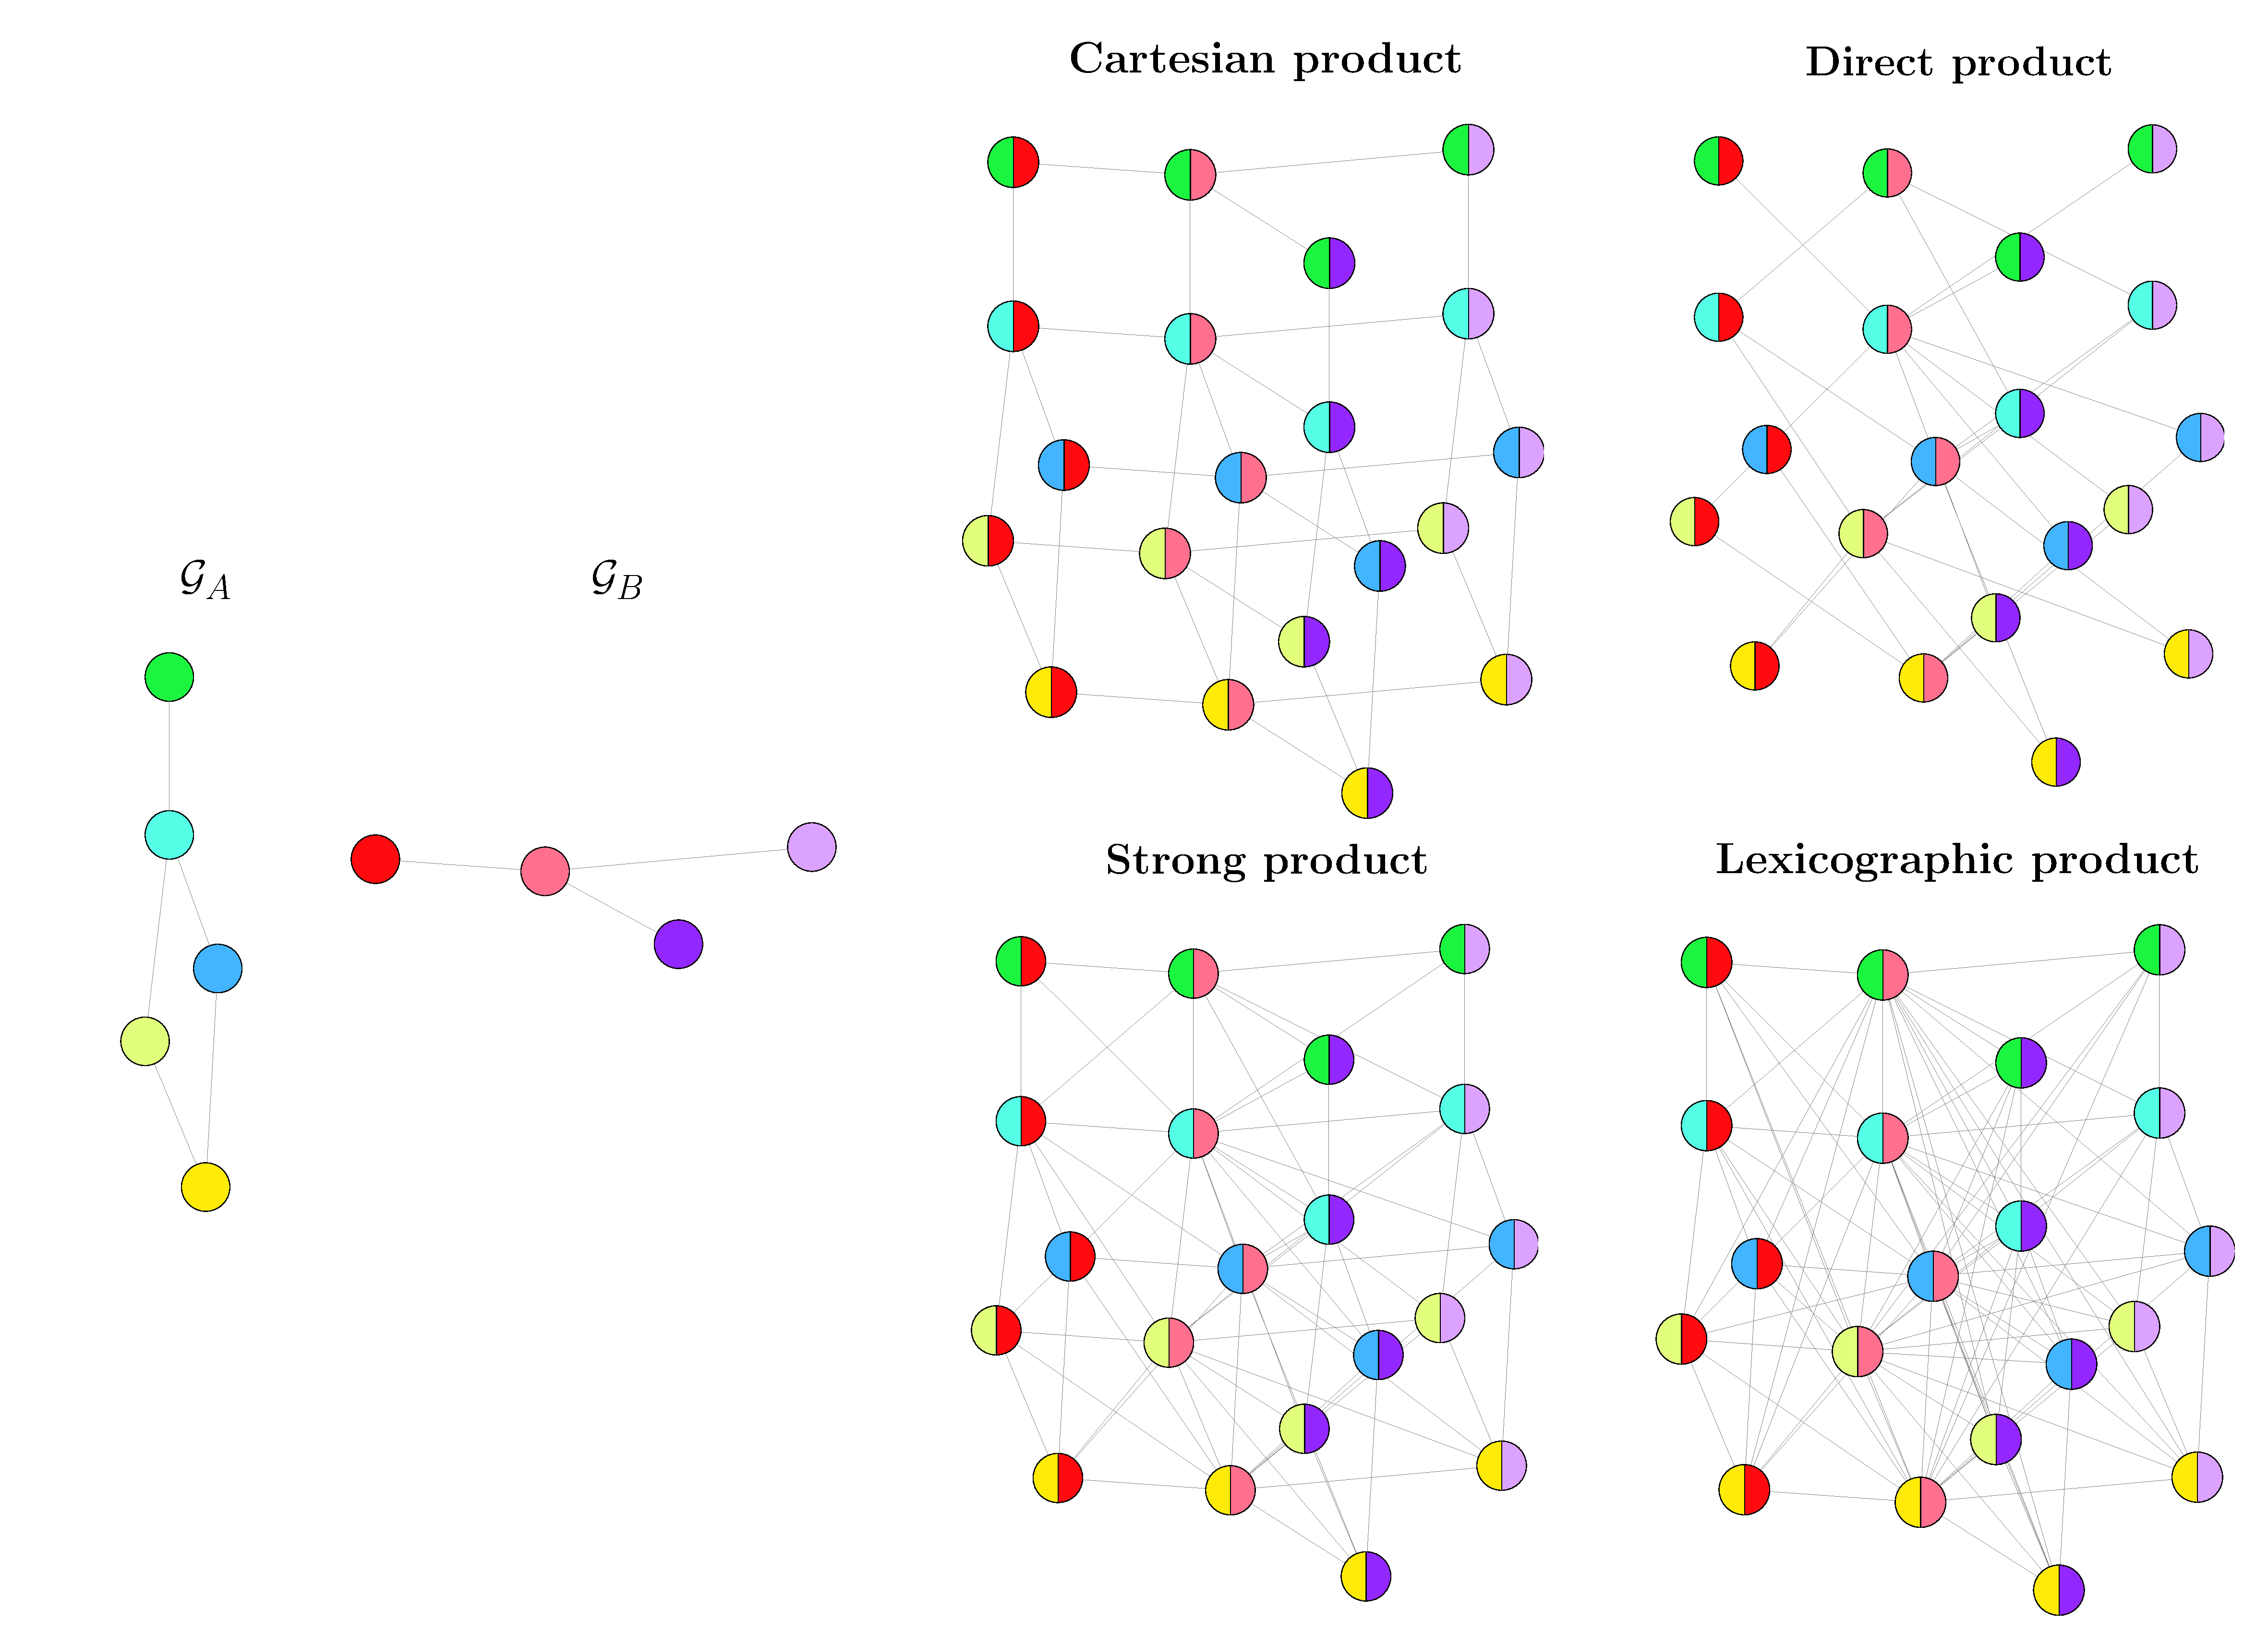
\includegraphics[width=0.95\linewidth]{Figures/product_graphs.pdf}
    \end{center}
    \caption[Graphical depiction of the standard graph products]{A graphical depiction of the four standard graph products}
    \label{fig:graph_products}
\end{figure}

% choice of product effect the sparsity or A/cardinality of V

% What is the natural 256 ordering in terms of sparsity

% make small example in terms of vertex order

Given these definitions, it may seem that all the standard graph products are non-commutative in the sense that $\A_A \oplus \A_B  \neq \A_B \oplus \A_A $ etc. However, the graphs $\mathcal{G}_A \, \diamond \, \mathcal{G}_B$ and $\mathcal{G}_B \, \diamond \, \mathcal{G}_A$ are in fact isomorphically identical in the case of the Cartesian, direct and strong products. This is not the case for the Lexicographic product \citep{Imrich2000}.

\subsection{The spectral properties of graph products}

In the field of graph signal processing, we are often concerned with analysing the properties of graphs via eigendecomposition of the graph Laplacian \citep{Mieghem2010}. In the case of product graphs, it is greatly preferable if we can fully describe the spectrum of $\mathcal{G}_A \diamond \mathcal{G}_B$ in terms of the spectra of $\mathcal{G}_A$ and $\mathcal{G}_B$ alone. This is because the direct decomposition of a dense $\LL$ has time-complexity $O(N_A^3N_B^3)$, whereas decomposition of the factor Laplacians individually has complexity $O(N_A^3 + N_B^3)$. As the graphs under consideration become medium to large, this fact quickly makes direct decomposition of the product graph Laplacian intractable. However, in the general case, only the spectra of the Cartesian and lexicographic graph products can be described in this way \citep{Barik2018}. In the case of the direct and strong product, it is possible to estimate the spectra without performing the full decomposition (see \citep{Sayama2016}). However, in general, the full eigendecomposition of the product graph Laplacian can only be described in terms of the factor eigendecompositions when both factor graphs are regular.


Consider the eigendecompositions of $\LL_A$ and $\LL_B$.

\begin{equation}
    \LL_A = \U_A \LAM_A \U_A^\top, \aand \LL_B = \U_B \LAM_B \U_B^\top
\end{equation}

where $\U_A$ and $\U_B$ are the respective orthonormal eigenvector matrices, and $\LAM_A$ and $\LAM_B$ are the diagonal eigenvalue matrices given by

\begin{equation*}
    \LAM_A = \diag{\begin{bmatrix} \lambda_1^{(A)}, & \lambda_2^{(A)}, & \dots & \lambda_A^{(A)} \end{bmatrix}},
    \aand
    \LAM_B = \diag{\begin{bmatrix} \lambda_1^{(B)}, & \lambda_2^{(B)}, & \dots & \lambda_B^{(B)} \end{bmatrix}}
\end{equation*}

Given these definitions, table \ref{tab:product_graph_spectra} gives information about the spectral decomposition of the standard graph products.

\begin{table}[t]
    \def\arraystretch{2}
    \centering
    \small
    \vspace{0.5cm}
    \begin{tabular}{l c c}
        \toprule

         & Eigenvalues
         & Eigenvectors                                                                          \\

        \midrule

        Cartesian
         & $\lambda_a^{(A)} + \lambda_b^{(B)}$
         & $(\U_A)_a \otimes (\U_B)_b$                                                           \\

        Direct$^{\star}$
         & $r_A \lambda_b^{(B)} + r_B \lambda_a^{(A)} - \lambda_a^{(A)} \lambda_b^{(B)}$
         & $(\U_A)_a \otimes (\U_B)_b$                                                           \\

        Strong$^{\star}$
         & $(1+r_A) \lambda_b^{(B)} + (1+r_B) \lambda_a ^{(A)}- \lambda_a^{(A)} \lambda_b^{(B)}$
         & $(\U_A)_a \otimes (\U_B)_b$                                                           \\

        \multirow{2}{7em}{Lexicographic$^\dagger$}
         & $N_B \lambda_a^{(A)}$
         & $(\U_A)_a \otimes \mathbf{1}_B$                                                       \\

         & $\lambda_b^{(B)} + N_B \text{deg}(a)$
         & $\mathbf{e}_a \otimes (\U_B)_b$                                                       \\

        \bottomrule
    \end{tabular}
    \vspace{0.2cm}
    \caption[Spectral decomposition of product graphs]{Eigendecomposition of the Laplacian of the standard graph products. Here, $a$ and $b$ are understood to run from 1 to $N_A$ and 1 to $N_B$ respectively. $\star$ only for $r_A$ and $r_B$-regular factor graphs. $\dagger$ note that the $b$ runs from 2 to $N_B$ in the lower row. }
    \vspace{0.3cm}
    \label{tab:product_graph_spectra}
\end{table}

% remark common degree locally only necessary 
% subspace concentration 


\subsection{GSP with Cartesian product graphs}

\label{sec:gsp_cpg}

While both the direct and strong products do find uses in certain applications (for example, see \citep{Kaveh2011}), they are both less common and more challenging to work with in a graph signal processing context due to their spectral properties described in the previous subsection. In practice, being limited to regular factor graphs means the majority of practical GSP applications are ruled out. The lexicographic product does not share this drawback, however, it is also significantly less common than the Cartesian product in real-world applications. For this reason, in the following, we focus primarily on the Cartesian product.

Given the spectral decomposition of the Cartesian graph product stated in table \ref{tab:product_graph_spectra}, we can write the Laplacian eigendecomposition in matrix form as follows.

\begin{equation}
    \LL = \U \LAM \U^\top, \where \U = \U_A \otimes \U_B \aand \LAM = \LAM_A \oplus \LAM_B
\end{equation}

This motivates the following definitions for the Graph Fourier Transform (GFT) and its inverse (IGFT). Consider a signal defined over the nodes of a Cartesian product graph expressed as a matrix $\Y \in \R^{N_B \times N_A}$. We can perform the GFT as follows.


\begin{equation}
    \label{eq:GFT_2d}
    \text{GFT}(\Y) = \mat{\big( \U_A^\top \otimes \U_B^\top \big) \, \vecc{\Y}} = \U_B^\top \Y \U_A
\end{equation}

Correspondingly, we can define the IGFT acting on a matrix of spectral components $\Z \in \R^{N_B \times N_A}$ as follows.

\begin{equation}
    \label{eq:IGFT_2d}
    \text{IGFT}(\Z) = \mat{\big( \U_A \otimes \U_B \big)\,\vecc{\Z}} = \U_B \Z \U_A^\top
\end{equation}


\note{Product graph signals: representation and vectorisation}{

    It is natural to assume that signals defined on the nodes of a Cartesian product graph $\mathcal{G}_A \, \square \; \mathcal{G}_B$ could be represented by matrices (order two tensors) of shape $(N_A \times N_B)$. Since product graph operators, such as the Laplacian $\LL_A \oplus \LL_B$, act on vectors of length $N_A N_B$, we must define a consistent function to map matrix graph signals $\in \R^{N_A \times N_B}$ to vector graph signals $\in \R^{N_A N_B}$. The standard mathematical operator for this purpose is the $\vecc{\cdot}$ function, along with its reverse operator $\mat{\cdot}$. However, this is somewhat problematic since $\vecc{\cdot}$ is defined to act in \textit{column-major} order, that is

    $$
        \text{vec} \left( \begin{bmatrix}
                \Y_{(1, 1)} & \Y_{(1, 2)} & \dots  & \Y_{(1, N_B)} \\
                \Y_{(2, 1)} & \Y_{(2, 2)} & \dots  & \Y_{(2, N_B)} \\
                \vdots      & \vdots      & \ddots & \vdots      \\
                \Y_{(N_A, 1)} & \Y_{(N_A, 2)} & \dots  & \Y_{(N_A, N_B)} \\
            \end{bmatrix} \right)
        =
        \begin{bmatrix}
            \Y_{(1, 1)} \\ \Y_{(2, 1)} \\ \vdots \\ \Y_{(N_A-1, N_B)} \\ \Y_{(N_A, N_B)}
        \end{bmatrix}
    $$

    As is visible, this does not result in a lexicographic ordering of the matrix elements when the graph signal has shape $(N_A \times N_B)$. Therefore, to avoid this issue and to be consistent with standard mathematical notation, we will assume that graph signals are represented by matrices of shape $(N_B \times N_A)$ when considering the product between two graphs $\mathcal{G}_A \, \square \, \mathcal{G}_B$. For graph signals of this shape, the first index represents traversal of the nodes in $\mathcal{G}_B$, and the second index represents traversal of the nodes in $\mathcal{G}_A$. This ensures that matrix elements are correctly mapped to vector elements when using the column-major $\vecc{\cdot}$ function.

}

Given these definitions, we can define a spectral operator (usually a low-pass filter) $\HH$ which acts on graph signals according to a spectral scaling function $g(\lambda \,; \, \beta)$ such as one of those defined in table \ref{tab:iso_filters}. As with regular non-product graphs, the action of this operator can be understood as first transforming a signal into the Laplacian frequency domain via the GFT, then scaling the spectral components according to some function, and finally transforming back into the vertex domain via the IGFT.

\begin{align}
    \label{eq:graph_filter}
    \HH & = g(\LL_A \oplus \LL_B) \notag                                                                                          \\
        & = \big( \U_A \otimes \U_B \big) \, g \big( \LAM_A \oplus \LAM_B \big) \, \big( \U_A^\top \otimes \U_B^\top \big) \notag \\
        & = \big( \U_A \otimes \U_B \big) \, \diag{\vecc{\G}} \, \big( \U_A^\top \otimes \U_B^\top \big) \notag \\
        &= \U \D_\G \U^\top
\end{align}

% remark which section of the thesis the properties of G are explained

The matrix $\G \in \R^{N_B \times N_A}$, which we refer to as the spectral scaling matrix, holds the value of the scaling function applied to the sum of
pairs of eigenvalues, such that

\begin{equation}
    \label{eq:Gba}
    \G_{ba} = g\left(\lambda^{(A)}_a + \lambda^{(B)}_b; \beta\right)
\end{equation}


% remark about Cartesian product eig sum

We observe that defining the filtering operation in this manner implies that the intensity is equal across both $\mathcal{G}_A$ and $\mathcal{G}_B$. We refer to filters of this type as \textit{isotropic}. This can be further generalised by considering an \textit{anisotropic} graph filter, which offers independent control over the filter intensity in each of the two dimensions. In this case, we define $\G$ as follows.

\begin{equation}
    \label{eq:Gba2}
    \G_{ba} =  g \left(\lambda^{(A)}_a, \lambda^{(B)}_b; \, \beta_a, \beta_b\right)
\end{equation}

where now $g$ is chosen to be an anisotropic graph filter such as one of those listed in table \ref{tab:anis_filters_2d}. Note that the original parameter $\beta$ is now replaced by two parameters $\beta_a$ and $\beta_a$ which offer control over the filter intensity in each dimension. Filters of this kind appear often in image processing literature \citep{Aubert2006}, however, their use in graph signal processing is so far limited. In \cite{Romero2017}, the authors propose `space-time kernels', which are related but specific to T-V problems. Our formulation, by contrast, is applicable to general two-dimensional Cartesian product graphs.  \Cref{fig:filters} depicts an anisotropic graph filter applied to an image, which is a special case of a 2D Cartesian product graph signal.  


\begin{table}[t]
    \vspace*{1cm}
    \def\arraystretch{1.8}
    \begin{center}
        \begin{tabular}{lc}
        \toprule
        \textbf{Filter}   & $g(\lambda_a, \lambda_b; \,\beta_a, \beta_b)$  \\
        \midrule
        1-hop random walk & $(1 + \beta_a \lambda_a + \beta_b \lambda_b)^{-1}$\\
        Diffusion         & $\exp(-\beta_a \lambda_a - \beta_b \lambda_b)$\\
        ReLu              & $\max (1 - \beta_a \lambda_a - \beta_b \lambda_b, 0)$ \\
        Sigmoid           & $2 \big( 1 + \exp(\beta_a \lambda_a + \beta_b \lambda_b)\big)^{-1}$\\
        Gaussian          & $\exp \big(-(\beta_a \lambda_a + \beta_b \lambda_b)^2\big)$\\
        Bandlimited       & $1, \,\text{if} \; \beta_a \lambda_a + \beta_b \lambda_b\leq 1 \; \text{else} \; 0$ \\
        \bottomrule
        \end{tabular}
    \end{center}
    \caption{Anisotropic graph filter functions in two dimensions}
    \label{tab:anis_filters_2d}
    \vspace*{1cm}
\end{table}


\begin{figure}[t]
    % \begin{center}
    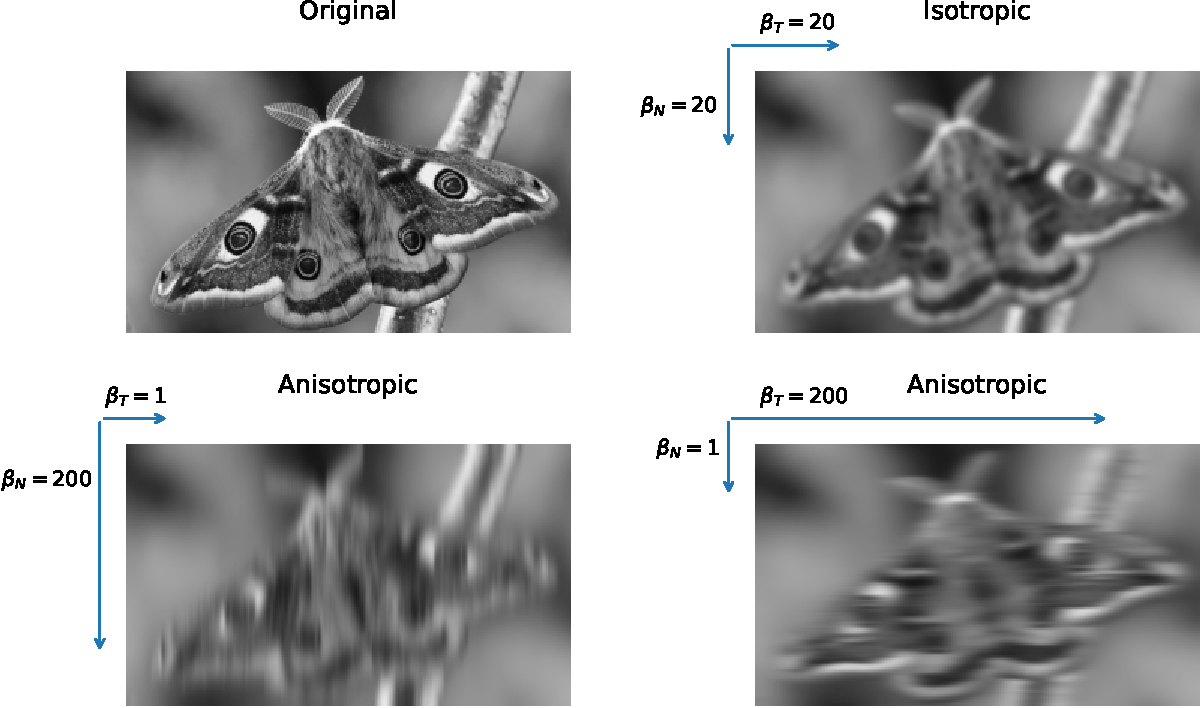
\includegraphics[width=0.9\linewidth]{Figures/filter_types_butterfly.pdf}
    % \end{center}
    \caption[A visual representation of applying an isotropic and anisotropic graph filter]{A visual representation of applying an isotropic and anisotropic graph filter. Here, the graph signal is an image, which can be thought of as existing on the nodes of a Cartesian product graph constructed by taking the product of two chain graphs. }
    \label{fig:filters}
\end{figure}



\section{Graph Signal Reconstruction on Cartesian Product Graphs}

\label{sec:gsr_cpg}

We now turn our attention to the task of signal reconstruction on Cartesian product graphs. In the following, we will replace the factor graph labels $A$ and $B$ with $T$ and $N$ respectively. The reason for this is that one application of particular interest is graph time-series problems, where we seek to model a network of $N$ nodes across a series of $T$ discrete time points. These so-called ``time-vertex'' (T-V) problems have garnered significant interest recently in the context of GSP \citep{Grassi2018, Isufi2017, Loukas2016}. T-V signals can be understood as existing on the nodes of a Cartesian product graph $\mathcal{G}_T \, \square \, \mathcal{G}_N$. In particular, we can conceptualise $T$ repeated measurements of a signal defined across the nodes of a $N$-node graph as a single measurement of a signal defined on the nodes of $\mathcal{G}_T \, \square \, \mathcal{G}_N$, where $\mathcal{G}_T$ is a simple path graph.

\vspace{1cm}


\begin{figure}[t]
    \begin{center}
        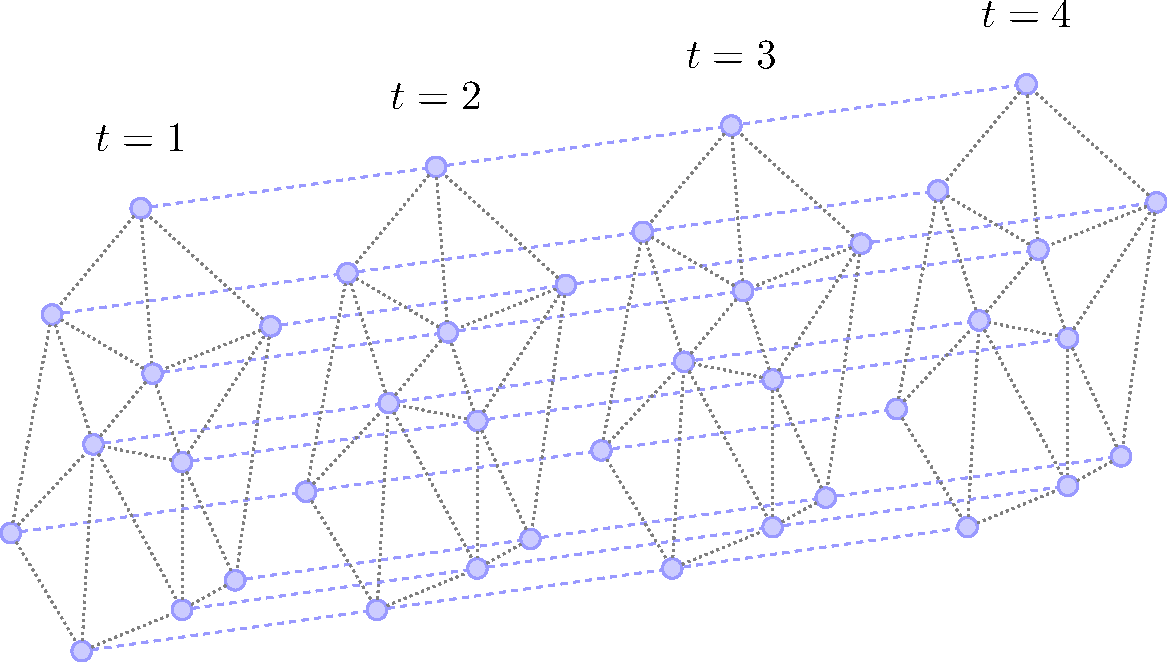
\includegraphics[width=0.75\linewidth]{Figures/TV.pdf}
    \end{center}
    \caption[A time-vertex Cartesian product graph]{A graphical depiction of a time-vertex Cartesian product graph. }
    \label{fig:TV}
\end{figure}



\note{On the Laplacian spectrum of the path graph}{
    \label{box}
    When considering time-vertex problems with uniformly spaced time intervals, $\mathcal{G}_T$ will be described by a path graph with equal weights on each edge. This special case of a graph has vertices given by $\mathcal{V}_T = \{t \in \mathbb{N} \, | \, t \leq T \}$ and edges given by $\mathcal{E}_T = \{ \, [t, t+1] \, | \, t < T \}$. The Laplacian matrix of the path graph is therefore given by

    $$
        \LL_T = \begin{bmatrix}
            1  & -1 &        &    &    \\
            -1 & 2  & -1     &    &    \\
               &    & \ddots &    &    \\
               &    & -1     & 2  & -1 \\
               &    &        & -1 & 1  \\
        \end{bmatrix}
    $$

    The eigenvalues and eigenvectors of this Laplacian are well-known and can be expressed in closed-form \citep{Jiang2012}. In particular,

    $$
        \lambda^{(T)}_t = 2 - 2 \cos \Big(  \, \frac{t - 1}{T} \pi \, \Big)
    $$

    and

    $$
        (\U_T)_{ij} = \cos \Big( \, \frac{j - 1}{T}\big(i - \frac{1}{2}\big)\pi \, \Big)
    $$

    where the columns of $\U$ are appropriately normalised such that the magnitude of each eigenvector is one. Furthermore, this implies that that the graph Fourier transform of a signal $\y \in \R^{T}$ is given by the orthogonal type-II Discrete Cosine Transform (DCT) \citep{Ahmed1974}. This is of significance, as it means we can leverage Fast Cosine Transform (FCT) algorithms \citep{Makhoul1980} which operate in a similar manner to the well-known Fast Fourier Transform (FFT) \citep{Cooley1965}. See chapter 4 of \cite{Rao1990} for an overview of FCT algorithms. In general, FFT-type algorithms are challenging to derive for the GFT \citep{LeMagoarou2016}, however, this is a simple case where it can be achieved. 

    \vspace{0.2cm}

    In particular, this reduces both of the following procedures

    \begin{equation*}
        \text{GFT}(\y) = \U_T^\top \y \aand \text{IGFT}(\y) = \U_T \y
    \end{equation*}

    from $O(T^2)$ operations to $O(T \log T)$ operations, which can be significant for large time-series problems. The figure below compares the time to compute the graph Fourier transform of a random signal using the matrix multiplication method vs the FCT implementation. In particular, we varied $T$ from 10 to 15,000 in 20 equally spaced increments and measured the mean time to compute $\U_T^\top \y$ across five independent trials using both the standard matrix multiplication and the Fast Cosine Transform method. As is visible, the difference becomes extremely pronounced as $T$ grows large.

    \begin{center}
        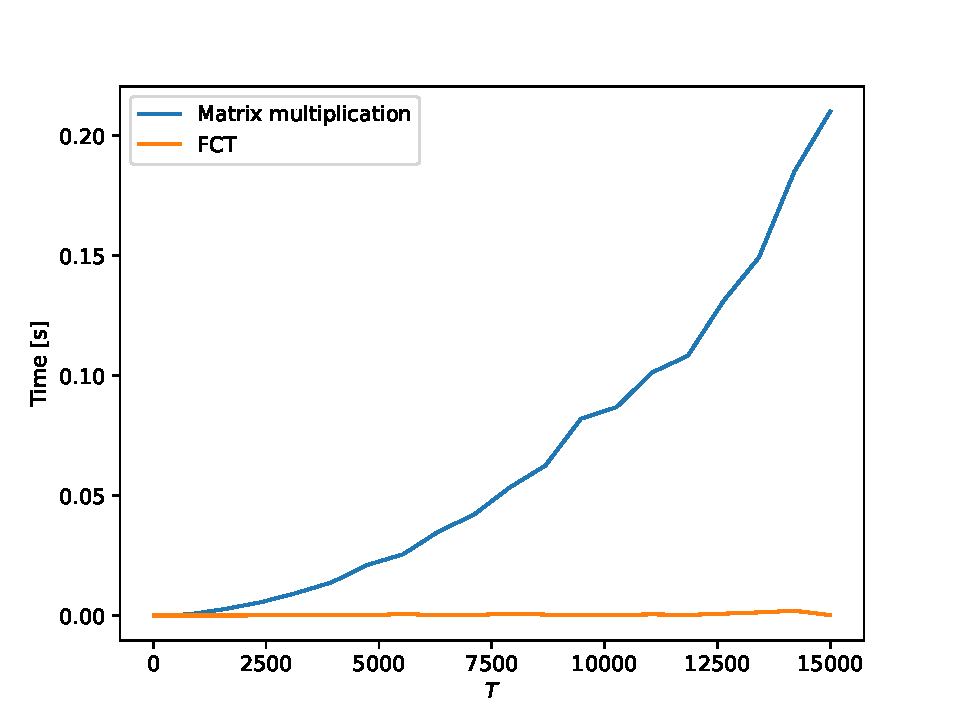
\includegraphics[width=0.9\linewidth]{Figures/DCT.pdf}
    \end{center}

    % write algorithm explicitly
    % what is aliasing in this context? 
    % Nyquist for GFT? 


}



Note that, despite the observation that $\mathcal{G}_T$ is often a path graph in the context of T-V problems, the methods introduced in this section are valid for the Cartesian product between arbitrary undirected factor graphs.

\subsection{Problem statement}

\label{sec:problem_statement_2d}


The goal of Graph Signal Reconstruction (GSR) is to estimate the value of a partially observed graph signal at nodes where no data was collected. In the context of GSR on a Cartesian product graph, the available data is an observed signal $\Y \in \R^{N \times T}$ where only a partial set $\mathcal{S} = \{(n_1, t_1), (n_2, t_2), \dots \}$ of the signal elements were recorded. All other missing elements of $\Y$ are set to zero. To track which elements were missing from $\Y$, we also define $\Ss \in \{0, 1\}^{N \times T}$, which is referred to as the binary sensing matrix. It has entries given by

\begin{equation}
    \Ss_{nt} = \begin{cases}
        1 & \text{if} \;\; (n, t) \in \mathcal{S} \\
        0 & \text{otherwise}
    \end{cases}
\end{equation}

As such, the data available for input into the GSR problem is as follows. 

\begin{equation*}
    \text{input data} = \Big\{\; \Y \in \R^{N \times T}, \;\; \Ss \in \{0, 1\}^{N \times T} , \;\; \A \in \R^{NT \times NT} \; \Big\}
\end{equation*}

Our model is based on the assumption that $\Y$ is a noisy partial observation of an underlying signal $\F \in \R^{N \times T}$, which is assumed to be smooth with respect to the graph topology. Specifically, we assume that the observed matrix $\Y$ is generated according to the following statistical model. 

\begin{equation}
    \Y = \Ss \circ \big(\F + \E \big)
\end{equation}

The matrix $\E$ represents the model error and is assumed to have an independent normal distribution with unit variance. Therefore, the probability distribution of $\Y$ given the latent signal $\F$ is

\begin{equation}
    \label{eq:Y_given_F}
    \vecc{\Y} \, | \, \F \sim \mathcal{N}\Big(\vecc{\Ss \circ \F}, \; \diag{\vecc{\Ss}}\Big)
\end{equation}

Note that the covariance matrix $\diag{\vecc{\Ss}}$ is semi-positive definite by construction. This naturally reflects the constraint that some elements of $\Y$ are zero with probability 1. 

In order to estimate the latent signal $\F$, we must provide a prior distribution describing our belief about its likely profile ahead of time. In general, we expect $\F$ to be smooth with respect to the topology of the graph. This can be expressed by setting the covariance matrix in its prior to be proportional to $\HH^2$, where $\HH$ is a graph filter as defined in equation (\ref{eq:graph_filter}). For now, in the absence of any further information, we assume that the prior mean for $\F$ is zero across all elements.

\begin{equation}
    \label{eq:F_prior}
    \vecc{\F} \sim \mathcal{N}\big(\zero, \, \gamma^{-1} \HH^2\big)
\end{equation}

Next, given an observation $\Y$, we use Bayes' rule to find the posterior distribution over $\F$. This is given by

\begin{equation}
    \pi\big(\vecc{\F} \, | \, \Y \big) = \frac{\pi\big(\vecc{\Y} \, | \, \F \big) \pi(\F) }{\pi(\Y)}.
\end{equation}

where we use the notation $\pi(\cdot)$ to denote a probability density function.

The posterior distribution for $\F$ is given by

\begin{equation}
    \label{eq:F_post_gsr}
    \vecc{\F} \, | \, \Y \sim \mathcal{N} \big(\PP^{-1} \, \vecc{\Y}, \; \PP^{-1} \big)
\end{equation}

\noindent where $\PP$ is the posterior precision matrix, given by 

\begin{equation}
    \label{eq:P_post_gsr}
    \PP = \diag{\vecc{\Ss}} + \gamma  \HH^{-2}
\end{equation}

A proof of this can be found in the appendix, theorem \ref{the:F_posterior}. In this chapter, we are primarily interested in computing the posterior mean, which is the solution to the following linear system.

\begin{equation}
    \label{eq:lin_system}
    \vecc{\F} = \Big(\diag{\vecc{\Ss}} + \gamma  \HH^{-2}\Big)^{-1} \vecc{\Y}
\end{equation}

We return to the question of sampling from the posterior and estimating the posterior covariance directly in \cref{chap:variance}.

Two significant computational challenges arise when working with non-trivial graph signal reconstruction problems, where the number of vertices in the product graph is large. First, although the posterior mean point estimator given in \cref{eq:lin_system} has an exact closed-form solution, its evaluation requires solving an $NT \times NT$ system of equations, which is impractical for all but the smallest of problems. Second, since the eigenvalues of $\HH$ can be close to or exactly zero, $\HH^{-2}$ may be severely ill-conditioned and even undefined. This means the condition number of the coefficient matrix may not be finite, making basic iterative methods to numerically solve the linear system, such as steepest descent, slow or impossible. The models proposed in this paper aim to overcome these problems.


Since the coefficient matrix defining the system is of size $NT \times NT $, direct methods such as Gaussian elimination are assumed to be out of the question. In such cases, one often resorts to one of three possible solution approaches: stationary iterative methods; Krylov methods; and multigrid methods. Each is part of the family of iterative methods which are most commonly found in applications of sparse matrices, such as finite element methods \citep{Brenner2008}. In the following, we propose a stationary iterative method and a Krylov method and compare their relative behaviour. In both cases, we show that each step of the iterative process can be completed in $O(N^2T + NT^2)$ operations, making a solution feasible for relatively large graph problems. First, we present each of the methods in isolation. Then, the convergence behaviour of each is derived theoretically and verified numerically.


\subsection{A stationary iterative method}

\label{sec:SIM}

In this section, we demonstrate a technique for obtaining the posterior mean by adopting a classic approach to solving linear systems, known as \textit{matrix splitting}, which sits within the family of Stationary Iterative Methods (SIMs) \citep{Saad2003}. The general splitting strategy is to break the coefficient matrix into the form $\M - \N$, such that 


\begin{equation}
    \vecc{\F} = (\M - \N)^{-1} \vecc{\Y}
\end{equation}

By noting that

\begin{align}
    \M \vecc{\F} &= \N \vecc{\F} + \vecc{\Y} \\
    \vecc{\F} &= \M^{-1}\N \vecc{\F} + \M^{-1} \vecc{\Y}
\end{align}

we devise an iterative scheme given by 

\begin{equation}
    \label{eq:sim_update}
    \vecc{\F_{k+1}} = \M^{-1}\N \vecc{\F_{k}} + \M^{-1} \vecc{\Y}
\end{equation}


When $\M$ is a simple matrix that is easy to invert, this update function can be vastly more efficient to compute. Common approaches to finding a suitable value for $\M$ and $\N$ include the Jacobi, Gauss-Seidel and successive over-relaxation methods, each of which represents a different strategy for splitting the coefficient matrix \citep{Saad2003}. However, whilst these techniques are well-studied, they are not appropriate for use in the case of graph signal reconstruction. This is because, for each of these methods, the coefficient matrix is split according to its diagonal and off-diagonal elements in some way. Consequently, this would require the evaluation of $\HH^{-2}$ directly which, as we have discussed, may be large, severely ill-conditioned and possibly ill-defined. 


Instead, we require a custom splitting that avoids direct evaluation of $\HH^{-2}$, and allows the right-hand side of \cref{eq:sim_update} to be computed efficiently. The main contribution of this subsection is the identification of appropriate values for $\M$ and $\N$, and an investigation of the consequences of that choice. 

In the following, we set 

\begin{equation}
    \M = \gamma \HH^{-2} + \I_{NT}, \aand \N = \diag{\vecc{\Ss'}}.
\end{equation}

where $\Ss'$ is the binary matrix representing the complement of the set of selected nodes, i.e.

\begin{equation}
    \label{eq:S_}
    \Ss'_{nt} = \begin{cases}
        1 & \text{if} \;\; (n, t) \notin \mathcal{S} \\
        0 & \text{otherwise}
    \end{cases}
\end{equation}

In this way, the update equation is given by 

\begin{equation}
    \label{eq:sim_update2}
    \vecc{\F_{k+1}} = \big(\gamma \HH^{-2} + \I \, \big)^{-1}  \diag{\vecc{\Ss'}} \vecc{\F_{k}} + \big(\gamma \HH^{-2} + \I \, \big)^{-1} \vecc{\Y}
\end{equation}



Note that this splitting is valid since $\big(\gamma\HH^{-2} + \I \, \big)^{-1}$ is guaranteed to exist. It can also be readily computed as we already have the eigendecomposition of $\HH$. Noting the decomposed definition of $\HH$ given in \cref{eq:graph_filter}, this can be written as

\begin{align}
    \label{eq:M_inv}
    \M^{-1} & = \Big( \gamma \HH^{-2} + \I \, \Big)^{-1} \notag \\
            & = \Big( \gamma \big(\U_T \otimes \U_N\big)\, \diag{\vecc{\G}}^{-2}\,  \big(\U_T^\top \otimes \U_N^\top\big)  + \I \, \Big)^{-1} \notag   \\
            & = \big(\U_T \otimes \U_N\big)\, \Big( \gamma \, \diag{\vecc{\G}}^{-2}\,    + \I \, \Big)^{-1} \big(\U_T^\top \otimes \U_N^\top\big) \notag \\
            & = \big(\U_T \otimes \U_N\big)\, \diag{\vecc{\J}}\,  \big(\U_T^\top \otimes \U_N^\top\big)
\end{align}

\noindent where $\J \in \R^{N \times T}$ has elements defined by

\begin{equation}
    \label{eq:Jnt}
    \J_{nt} = \frac{\G_{nt}^2}{\G_{nt}^2 + \gamma}.
\end{equation}

Note that the update formula can be computed with $O(N^2T + NT^2)$ complexity at each step.  


\begin{align}
    \label{eq:update3}
    \F_{k+1} & = \U_N \, \big( \J  \circ \big( \U_N^\top \, (\Ss' \circ \F_{k})\, \U_T \big) \big) \, \U_T^\top + \F_0 \\
    \label{eq:update4}
    \text{with} \quad\quad\quad \F_0 & = \U_N \, \big( \J  \circ \big( \U_N^\top \, \Y \, \U_T \big) \big) \, \U_T^\top 
\end{align}


Furthermore, this is reduced to $O(N^2T + NT \log T)$ in the case of T-V problems, and to $O\big(NT \log NT \big)$ for data residing on a grid (see \cref{box}). 


It is well-known that a given splitting will be convergent if the largest eigenvalue $\lambda_{\text{max}}$ of the matrix $\M^{-1}\N$ has an absolute value of less than one. This attribute, $\rho = |\lambda_{\text{max}}|$, is known as the spectral radius. 

Whilst the spectral radius of $\M^{-1}\N$ cannot be computed directly, we can derive an upper bound based on the properties of $\M$ and $\N$ individually. 

Consider the spectral radius of $\M^{-1}$. By directly inspecting \cref{eq:M_inv}, it is clear that $\rho(\M^{-1})$ will be the maximum entry in the matrix $\J$ since $\M^{-1}$ is already diagonalised in the basis $\U_T \otimes \U_N$. Consider now the definition of $\J$ given in \cref{eq:Jnt}. By definition, $g(\cdot)$ has a maximum value of one on the non-negative reals, achieved when its argument is zero. Since the graph Laplacian is guaranteed to have at least one zero eigenvalue, the maximum entry in the matrix $\J$, and therefore the spectral radius of $\M^{-1}$, is surely given by

\begin{equation}
    \rho(\M^{-1}) = \frac{1}{1 + \gamma}
\end{equation}

Next, consider the spectral radius of $\N$. This can be extracted directly as one since it is a diagonal binary matrix. Since both $\M^{-1}$ and $\N$ are positive semi-definite, we can apply the theorem

\begin{equation}
    \label{eq:psd}
    \rho(\A\B) \leq \rho(\A) \, \rho(\B)
\end{equation}

\citep{Bhatia1997}. Therefore, the spectral radius of $\M^{-1}\N$ is guaranteed to be less than or equal to $1 / (1 + \gamma)$.  Since $\gamma$ is strictly positive, this is less than one and, as such, convergence is guaranteed. We return to the question of convergence more thoroughly in \cref{sec:convergence}. 

Finally, the update formulas given in \cref{eq:update3,eq:update4} can be written equivalently as 

\begin{align}
    \Delta \F_0     & = \U_N \, \big( \J  \circ \big( \U_N^\top \, \Y \, \U_T \big) \big) \, \U_T^\top  \\
    \Delta \F_{k+1} & = \U_N \, \big( \J  \circ \big( \U_N^\top \, (\Ss' \circ \Delta \F_{k})\, \U_T \big) \big) \, \U_T^\top
\end{align}

In this form, the iterations can be easily terminated when $|\Delta \F_{k}|$ is sufficiently small. The complete procedure is given in algorithm \hyperlink{al:SIM}{\textbf{1}}.

\begin{algorithm}[t]
    \hypertarget{al:SIM}{}
    \caption{Stationary iterative method with matrix splitting}
    \begin{algorithmic}
        \vspace{0.05cm}
        \Require{Observation matrix $\Y \in \R^{N \times T}$}
        \vspace{0.05cm}
        \Require{Sensing matrix $\Ss \in \{0, 1\}^{N \times T}$}
        \vspace{0.05cm}
        \Require{Space-like graph Laplacian $\LL_N \in \R^{N \times N}$}
        \vspace{0.05cm}
        \Require{Time-like graph Laplacian $\LL_T \in \R^{T \times T}$}
        \vspace{0.05cm}
        \Require{Regularisation parameter $\gamma \in \R^{+}$}
        \vspace{0.05cm}
        \Require{Graph filter function $g(\, \cdot\, \,; \betaa \in \R^{2})$}
        \vspace{0.15cm}
        \State{Decompose $\LL_N$ into $\U_N \LAM_L \U_N^\top$ and $\LL_T$ into $\U_T \LAM_T \U_T^\top$}
        \vspace{0.15cm}
        \State{Compute $\G \in \R^{N \times T}$ as $\G_{nt} = g \left(\lambda^{(N)}_n, \lambda^{(T)}_t; \, \betaa \right)$ }
        \vspace{0.15cm}
        \State{Compute $\J \in \R^{N \times T}$ as $\J_{nt} = \G_{nt}^2 / (\G_{nt}^2 + \gamma)$ }
        \vspace{0.15cm}
        \State{$\Ss' \leftarrow \mathbf{1} \in \R^{N \times T} - \Ss$}
        \vspace{0.15cm}
        \State{$\Delta\F \leftarrow \U_N\big( \J \circ (\U_N^\top \Y \U_T) \big)\U_T^\top$}
        \vspace{0.15cm}
        \State{$ \F  \leftarrow \Delta\F$}
        \vspace{0.15cm}
        \While{$|\Delta\F| > \text{tol}$}
        \vspace{0.15cm}
        \State{$\Delta\F \leftarrow \U_N \Big( \J \circ \big( \U_N^\top\, (\Ss' \circ \Delta\F ) \, \U_T \big) \Big) \U_T^\top$}
        \vspace{0.15cm}
        \State{$ \F \leftarrow  \F  + \Delta\F$}
        \vspace{0.15cm}
        \EndWhile
        \vspace{0.15cm}
        \Ensure{$ \F $}
        \vspace{0.15cm}
        \label{al:SIM}
    \end{algorithmic}
\end{algorithm}

\subsubsection{An eigendecomposition-free distributed implementation}

In the previous section, we introduced the SIM algorithm, premised on the assumption that the matrices $\LL_T$ and $\LL_N$ could be decomposed into $\U_T \LAM_T \U_T^\top$ and $\U_N \LAM_N \U_N^\top$ respectively. However, it is also feasible to implement the SIM in a manner that avoids the eigendecomposition of both Laplacians and instead only requires the repeated multiplication of vectors by $\LL_T \oplus \LL_N$ in the node domain. If, as is often the case, the original graphs are sparse, this can be achieved with complexity $O(T|\mathcal{E}_N| + N |\mathcal{E}_T|)$. This alternative is particularly beneficial when working with large factor graphs since the complexity involved in decomposition generally scales at $O(N^3 + T^3)$. 

Moreover, in certain contexts like sensor or IoT networks, nodes may possess the capability to communicate and compute locally. In such instances, a distributed approach to the signal reconstruction problem, employing a message-passing algorithm, may be more desirable. In this section, we will discuss how these two objectives can be realised by utilising Chebyshev polynomials \citep{Rivlin2020}.

First, note that each iteration of the SIM algorithm is computed by multiplying some vector, $\vecc{\Z}$, by the matrix $\M^{-1}$, which is given by \cref{eq:M_inv}. Crucially, since $\M^{-1}$ has eigenvectors $\U_T \otimes \U_N$, it can be understood as a function applied to a weighted Kronecker sum of the factor graph Laplacians. In particular, 

\begin{equation}
    \M^{-1} = J(\beta_T \LL_T \oplus \beta_N \LL_N)
\end{equation}

where 

$$
J(x) = \frac{g^2(x)}{g^2(x) + \gamma} 
$$

and $g(\cdot)$ represents the original filter function used, with parameters $\beta_T, \beta_N$. (Here, we interpret the application of $J(x)$ to a matrix in terms of a power series rather than element-wise.) Thus, eigendecomposition can be entirely bypassed by approximating the function $J(x)$ using shifted Chebyshev polynomials \citep{Isufi2022}. This requires knowledge of the largest eigenvalues of $\LL_T$ and $\LL_N$, $ \lambda_T^{(\text{max})}$ and $ \lambda_N^{(\text{max})}$ respectively, but these can also be computed efficiently using methods that take advantage of sparsity such as Arnoldi iterations.
 
Assuming an order $K$ approximation to the function $J(x)$ is used, with shifted Chebyshev polynomials ${\bar{T}_k(x)}$ defined over the interval $[0, \bar{\lambda}]$, where $\bar{\lambda} = \beta_T \lambda_T^{(\text{max})} + \beta_N \lambda_N^{(\text{max})}$,  the approximation is given by

\begin{equation}
    J(x) \approx \sum_{k=0}^K c_k \bar{T}_k(x)
\end{equation}

where the coefficients, $c_k$, are computed numerically via the integral given in \cref{eq:Cheb_int} of \cref{sec:Chebyshev}. The action of $\M^{-1}$ on an arbitrary vector $\vecc{\Z}$ can then be approximately computed as

\begin{equation}
    \M^{-1} \vecc{\Z} \approx \sum_{k=0}^K c_k \, \bar{T}_k(\bar{\LL}) \vecc{\Z} 
\end{equation}

where $\bar{\LL} = \beta_T \LL_T \oplus \beta_N \LL_N$. The result of $\bar{T}(\bar{\LL}) \vecc{\Z} $ is defined recursively as 

\begin{equation}
    \bar{T}_k(\bar{\LL}) \vecc{\Z} = \left(\frac{4 \bar{\LL}}{\bar{\lambda}} - 2\right) \bar{T}_{k-1}(\bar{\LL}) \vecc{\Z} -\bar{T}_{k-2}(\bar{\LL}) \vecc{\Z}
\end{equation}

with the initial conditions

\begin{equation}
    \bar{T}_0(\bar{\LL}) \vecc{\Z} = \vecc{\Z}, \aand \bar{T}_1(\bar{\LL}) \vecc{\Z} = \frac{2}{\bar{\lambda}} \bar{\LL} \vecc{\Z} - \vecc{\Z}
\end{equation}

In addition, the action of $\bar{\LL}$ on $\vecc{\Z}$ can be efficiently computed as

\begin{equation}
    \mat{\bar{\LL} \vecc{\Z}} = \beta_N \LL_N \Z + \beta_T \Z \LL_T 
\end{equation}

with complexity $O\big(NT(|\mathcal{E_T}| + |\mathcal{E}_N|)\big)$. When performed in a distributed manner, this operation can be executed at each node utilising information about the value of $\vecc{\Z}$ at its direct neighbours only. This implies that to compute an order $K$ polynomial, information will need to be gathered from nodes that are a maximum of $K$ hops away via graph edges. 

In the context of a graph time series problem, this method also lends itself to an online implementation. In particular, since each node requires information from nodes no further than $K$ hops away, the signal at node $n$ at time $t$ can be reconstructed when the observed signal at time $t+K$ becomes available. 

One caveat worth noting is that the accuracy of the Chebyshev approximation depends not only on the order of the polynomial but also on the filter used and its parameter(s). \Cref{fig:cheb_approx} demonstrates how an order-3 approximation to $J(x)$, with $\gamma=0.05$, varies across several different filter types and parameter settings. For filter functions that exhibit slow variation, typically corresponding to smaller values of $\beta$, the fit is usually quite accurate. However, in certain other contexts, it deviates significantly from the true filter function. Another consideration is that the spectral radius of $\M^{-1}$ is no longer guaranteed to be less than one. For instance, in the case of the bandlimited filter, the function clearly reaches higher values. To guarantee convergence, the polynomial coefficients should be adjusted such that the approximation remains within the range of $[-1, 1]$. 

\vspace{0.5cm}

\begin{figure}[t]
    \hspace{0.2cm}
        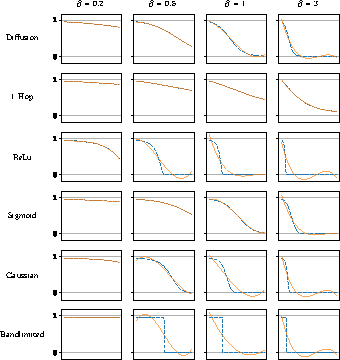
\includegraphics[width=0.9\linewidth]{Figures/cheb_approx.pdf}
    \caption[Chebyshev approximation accuracy visualisation]{\small{An order-3 Chebyshev polynomial approximation (orange) is compared to the true output of $J(x)$ (dashed blue) for several different filter types across various parameter settings. }}
    \label{fig:cheb_approx}
\end{figure}


\subsection{A conjugate gradient method}

\label{sec:CGM}

The second approach we consider for computing the posterior mean is to use the Conjugate Gradient Method (CGM). First proposed in 1952, the CGM is part of the Krylov subspace family and is perhaps the most prominent iterative algorithm for solving linear systems \citep{Hestenes1952}. In computational terms, the method only requires repeated forward multiplication of vectors by the coefficient matrix which, in the standard CGM, bust be PSD. It is therefore effective in applications where this process can be performed efficiently. 

In brief, the CGM seeks to solve the linear system $\A \x = \bb$ by minimising, at the $k$-th iteration, some measure of error in the affine space $\x_0 + \mathcal{K}_k$ where $\mathcal{K}_k$ is the $k$-th Krylov subspace given by  

$$
\mathcal{K}_k = \text{span}\big(\rr_0, \; \A \rr_0, \, ..., \, \A^{k-1} \rr_0 \big)
$$

The residual $\rr_k$ is given by 

$$
\rr_k = \bb - \A \x
$$

and the $k$-th iterate of the CGM minimises 

$$
\phi(\x) = \frac{1}{2} \x^\top \A \x  - \x^\top \bb
$$

over $\x_0 + \mathcal{K}_k$ \citep{Kelley1995}. 

The CGM works best when the coefficient matrix $\A$ has a low condition number $\kappa$ (that is, the ratio between the largest and smallest eigenvalue is small) and, as such, a preconditioning step is often necessary. The purpose of a preconditioner is to reduce $\kappa$ by solving an equivalent transformed problem. This can be achieved by right or left multiplying the linear system by a preconditioning matrix $\PSI$. However, this likely means the coefficient matrix is no longer PSD, meaning the CGM cannot be used in its basic form. (Other approaches modified for non-PSD matrices exist, e.g. the CGNE or GIMRES \citep{Elman1982, Saad1986}). A preconditioner can also multiply the coefficient matrix on the right by a preconditioner $\PSI^\top$ and on the left by $\PSI$. This preserves the symmetry meaning we can continue to use the regular CGM. 

In our case, where the coefficient matrix is given by $\Big(\diag{\vecc{\Ss}} + \gamma  \HH^{-2}\Big)$, preconditioning will be essential for convergence. To see why, consider the definition of $\HH$ in equation (\ref{eq:graph_filter}). A low-pass filter function $g(\cdot)$ may be close to zero when applied to the high-frequency eigenvalues of the graph Laplacian, meaning elements of $\diag{\vecc{\G}}^{-2}$ may be very large. In the worst case, for example with a band-limited filter, the matrix $\HH$ will be singular, no matrix $\HH^{-2}$ will exist, and the condition number of the coefficient matrix will be, in effect, infinite. Therefore, the primary purpose of this subsection is to find a preconditioner that maintains efficient forward multiplication and is effective at reducing the condition number of the coefficient matrix.

References such as \citep{Saad2003} give a broad overview of the known approaches to finding a preconditioner. Standard examples include the Jacobi preconditioner which is given by the inverse of the coefficient matrix diagonal and is effective for diagonally dominant matrices, and the Sparse Approximate Inverse preconditioner \citep{Grote1997}. However, such preconditioners generally require direct evaluation of parts of the coefficient matrix or are computationally intensive to calculate.

In the following, we derive an effective symmetric preconditioner that allows forward multiplication of the coefficient matrix to be performed efficiently. First consider the transformed variable $\Z$, related to $\F$ in the following way.

\begin{equation}
    \label{eq:Z_transform}
    \F = \U_N \, (\G \circ \Z) \, \U_T^\top
\end{equation}

Here, $\Z$ can be interpreted as a set of Laplacian frequency coefficients, which are subsequently scaled according to the graph filter function, and then reverse Fourier transformed back into the node domain. Matrices $\Z$ which are distributed according to a spherically symmetric distribution, result in signals $\F$ which are smooth with respect to the graph topology. Since this transform filters out the problematic high-Laplacian frequency Fourier components, the system defined by this transformed variable $\Z$ is naturally far better conditioned.

By substituting this expression for $\F$ back into the likelihood in equation (\ref{eq:Y_given_F}), and the prior of equation (\ref{eq:F_prior}), one can derive a new expression for the posterior mean of $\Z$. This is done explicitly in \cref{the:Z_transform_bayes}. The end result is that the new linear system for the transformed variable $\Z$ is given by


\begin{equation}
    \label{eq:Z_post}
    \vecc{\Z} = \Big( \D_{\G} \big( \U_T^\top \otimes \U_N^\top \big)\, \D_{\Ss} \, \big(\U_T \otimes \U_N \big) \,\D_{\G} + \gamma \I_{NT} \Big)^{-1} \vecc{\G \circ \big(\U_N^\top \Y \U_T\big)}
\end{equation}

\noindent where we have abbreviated $\diag{\vecc{\G}}$ and $\diag{\vecc{\Ss}}$ as $\D_{\G}$ and $\D_{\Ss}$ respectively. Note that the conditioning of the coefficient matrix is greatly improved from the untransformed problem, as we will discuss in greater detail in \cref{sec:convergence}. Note also that the multiplication of a vector $\vecc{\RR}$ by the coefficient matrix can be computed efficiently as 

\begin{multline}
    \mat{\Big( \D_{\G} \big( \U_T^\top \otimes \U_N^\top \big)\, \D_{\Ss} \, \big(\U_T \otimes \U_N \big) \,\D_{\G} + \gamma \I_{NT} \Big) \, \vecc{\RR}} \\ = \gamma \RR + \G \circ \left(\U_N^\top \Big( \Ss \circ \big(\U_N (\G \circ \RR) \U_T^\top \big) \Big) \U_T\right) 
\end{multline}



This has $O(N^2T + NT^2)$ complexity at each step which may be reduced to $O(N^2T + NT \log T)$ in the case of T-V problems, and to $O\big(NT \log NT \big)$ for data residing on a grid (see \cref{box}). 

The linear system defined \cref{eq:Z_post} can be understood as a two-sided symmetrically preconditioned version of the original linear system given in \cref{eq:lin_system}. In particular, the new expression can be constructed by modifying the original system in the following way.

\begin{equation}
    \Big(\PSI^\top  \big(\D_{\Ss} + \gamma  \HH^{-2}\big) \, \PSI  \Big) \Big(\PSI^{-1}\, \vecc{ \F } \Big) = \PSI^\top \, \vecc{\Y},
\end{equation}

\noindent where

\begin{equation}
    \PSI =   \big(\U_T \otimes \U_N\big) \, \D_{\G}.
\end{equation}

Since preconditioning of the coefficient matrix on the left is achieved with $\PSI^\top$ and on the right with $\PSI$, symmetry is preserved. This ensures that one can continue to utilise algorithms tailored to work with PSD matrices. In algorithm \hyperlink{al:CGM}{\textbf{2}}, we outline a conjugate gradient method based on this new formulation. 

\begin{algorithm}[t]
    \hypertarget{al:CGM}{}
    \label{al:MVGKR}
    \caption{Conjugate gradient method with graph-spectral preconditioner}
    \begin{algorithmic}
        \vspace{0.15cm}
        \Require{Observation matrix $\Y \in \R^{N \times T}$}
        \vspace{0.05cm}
        \Require{Sensing matrix $\Ss \in \{0, 1\}^{N \times T}$}
        \vspace{0.05cm}
        \Require{Space-like graph Laplacian $\LL_N \in \R^{N \times N}$}
        \vspace{0.05cm}
        \Require{Time-like graph Laplacian $\LL_T \in \R^{T \times T}$}
        \vspace{0.05cm}
        \Require{Regularisation parameter $\gamma \in \R$}
        \vspace{0.05cm}
        \Require{Graph filter function $g(\, \cdot\, \,; \betaa)$}
        \vspace{0.25cm}
        \State{Decompose $\LL_N$ into $\U_N \LAM_L \U_N^\top$ and $\LL_T$ into $\U_T \LAM_T \U_T^\top$}
        \vspace{0.15cm}
        \State{Compute $\G \in \R^{N \times T}$ as $\G_{nt} = g \left(\lambda^{(A)}_a, \lambda^{(B)}_b; \, \beta_a, \beta_b\right)$ }
        \vspace{0.15cm}
        \State{Initialise $\Z \in \R^{N \times T}$ randomly}
        \vspace{0.15cm}
        \State{$\RR \leftarrow \G \circ (\U_N^\top \Y \U_T) - \gamma \Z - \G \circ \Big( \, \U_N^\top \big(\Ss \circ (\U_N \, (\G \circ \Z) \, \U_T^\top) \big)  \, \U_T\Big)$}
        \vspace{0.15cm}
        \State{$\D \leftarrow \RR$}
        \vspace{0.15cm}
        \While{$|\Delta\RR| > \text{tol}$}
        \vspace{0.15cm}
        \State{$\A_D \leftarrow \gamma \D + \G \circ \Big( \, \U_N^\top \big(\Ss \circ (\U_N \, (\G \circ \D) \, \U_T^\top) \big)\, \U_T\Big) $}
        \vspace{0.15cm}
        \State{$\alpha \leftarrow  \tr{\RR^\top \RR} \, / \, \tr{\RR^\top \A_D \RR}$}
        \vspace{0.15cm}
        \State{$\Z \leftarrow  \Z + \alpha \D $}
        \vspace{0.15cm}
        \State{$\RR \leftarrow  \RR - \alpha \A_D $}
        \vspace{0.15cm}
        \State{$\delta \leftarrow \tr{\RR^\top \RR} \, / \, \tr{(\RR + \alpha \A_D)^\top (\RR + \alpha \A_D)}$}
        \vspace{0.15cm}
        \State{$\D \leftarrow  \RR + \delta \D $}
        \vspace{0.15cm}
        \EndWhile
        \vspace{0.25cm}
        \Ensure{$\U_N \, (\G \circ \Z) \, \U_T^\top$}
        \vspace{0.15cm}
    \end{algorithmic}
\end{algorithm}
 
\subsection{Real data experiments}

In this subsection, we evaluate our GSR method using a dataset consisting of daily new SARS-CoV-2 cases reported in 372 lower-tier local authorities across the United Kingdom from February 5, 2020, to March 18, 2023 (1138 days) taken from the UK government website\footnote{See \url{https://coronavirus.data.gov.uk/details/download}}. Specifically, we focused on the ``newCasesBySpecimenDateRollingRate" metric, which represents the daily number of cases reported per 100,000 residents in each local reporting authority over a 7-day rolling period. To create a graph, we used boundary data \footnote{Data from the Office for National Statistics \citep{ONS2019}}, setting adjacency matrix entries as $\A_{ij}$ = 1 if districts $i$ and $j$ share a border, and 0 otherwise. \Cref{fig:covid} illustrates a snapshot of this dataset on December 1, 2020.


\begin{figure}[b]
    \begin{center}
        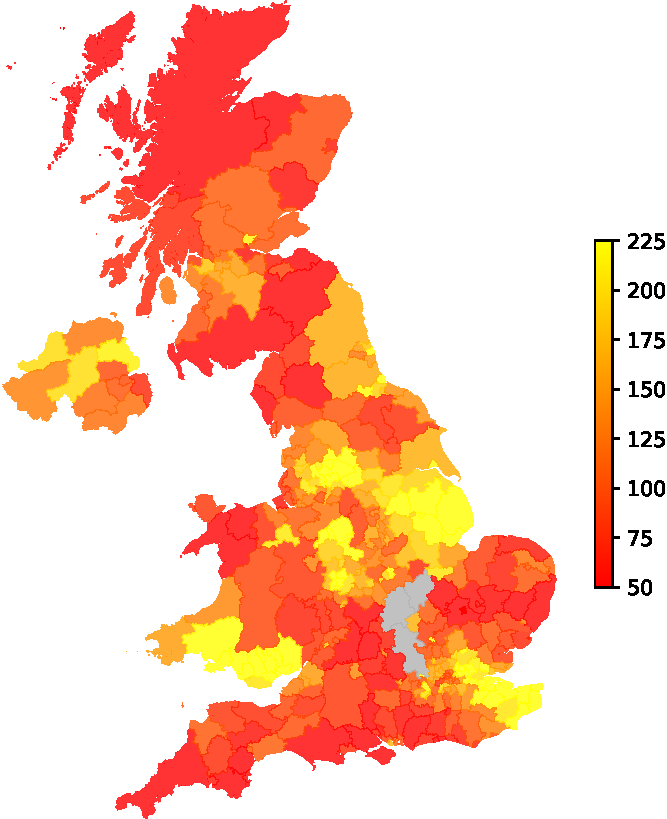
\includegraphics[width=0.6\linewidth]{Figures/UK_covid.pdf}
    \end{center}
    \caption[Snapshot of the Covid-19 case rate in the UK]{\small{The seven-day rolling rate of new covid cases reported per 100,000 residents in each lower-tier local reporting authority in the United Kingdom on the 1st of December 2020. Missing data is indicated in grey.}}
    \label{fig:covid}
\end{figure}


Before beginning the experiments, we performed two preprocessing steps on the raw signal data. First, we took the logarithm of 10 plus the original case rate. This was to eliminate the long tail in the case rate histogram, transforming it to be closer to a Gaussian. We then normalised by subtracting the overall mean and dividing by the standard deviation. The resultant signal, of shape $372 \times 1138$, we refer to as $\Y_0$. Note that 4.8\% of the entries in $\Y_0$ were already missing from the original dataset (mostly occurring in the earlier stages of the pandemic).

The experiment was conducted as follows. First, we removed data from $\Y_0$ such that a total fraction $m$ was no longer present. This created two matrices: $\Y$, the partially observed signal with missing values filled with zeros; and $\Ss$, the corresponding binary sensing matrix. Data was removed in four distinct ways. First, individual elements of $\Y$ were selected uniformly at random for removal (`uniform'). Second, strings of 100 days, beginning at a random date, were removed for individual randomly selected districts (`strings'). Third, the entire time series for randomly chosen districts were removed (`districts'). Finally, the signal across every node at randomly selected dates was removed (`dates'). These four techniques for data removal are depicted for clarity in \cref{fig:missing_data}. For each technique, we solved the signal reconstruction problem using the GSR model described in this chapter and compared its performance to other baseline reconstruction strategies. In particular, for uniform and string removal, we compared it to linear interpolation in time and longitudinal averaging across all districts. For date removal, we compared it to interpolation in time only, since longitudinal averaging is not possible in this case. Finally, for district removal, we compared it to longitudinal averaging, since linear interpolation in time is not possible in this case. For each model, for each method of data removal, we measured the Root Mean Square Error (RMSE) across the reconstructed entries, over four increasing values of $m$. The results are shown in \cref{tab:gsr_real_data_experiemnts}. 



\begin{figure}[t]
    \begin{center}
        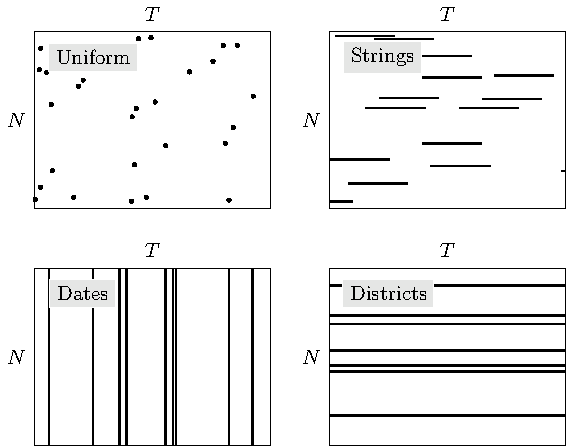
\includegraphics[width=0.6\linewidth]{Figures/missing.pdf}
    \end{center}
    \caption{\small{A visual depiction of the four ways we removed data. Black lines/dots indicate data that was removed. }}
    \label{fig:missing_data}
\end{figure}


\definecolor{best}{rgb}{0.6,0.99,0.58}


 
\begin{table*}[t]
    \centering
    \footnotesize 
    \def\arraystretch{1.4}
    \begin{tabular}{lcccccccccc}
    \toprule
    & \multicolumn{4}{c}{Uniform} & \phantom{a} & \multicolumn{4}{c}{Strings} \\
    \cmidrule{2-5} \cmidrule{7-10} 
    $m$ & 0.1   & 0.3 & 0.5 & 0.7 &&  0.1   & 0.3  & 0.5 & 0.7  \\ \midrule \rule{0pt}{0.5cm}
    GSR & 0.037 & 0.040 & \colorbox{best!35}{0.048} & 0.081 && \colorbox{best!35}{0.230} &  \colorbox{best!35}{0.249} & \colorbox{best!35}{0.247} & \colorbox{best!35}{0.243} \\ \rule{0pt}{6ex} 
    Linear interp & \colorbox{best!35}{0.034} & \colorbox{best!35}{0.039} &  \colorbox{best!35}{0.048} & \colorbox{best!35}{0.070} && 0.540 & 0.531 & 0.520 & 0.526 \\ \rule{0pt}{6ex}
    Longitudinal avrg & 0.350 & 0.348 &  0.347 & 0.348 && 0.341 & 0.350 & 0.356 & 0.347  \\[0.2cm] \midrule \rule{0pt}{4ex}
    & \multicolumn{4}{c}{Dates} & \phantom{a} & \multicolumn{4}{c}{Districts} \\
    \cmidrule{2-5} \cmidrule{7-10} 
    $m$ & 0.1   & 0.3 & 0.5 & 0.7 &&  0.1   & 0.3  & 0.5 & 0.7  \\ \midrule \rule{0pt}{0.5cm}
    GSR & 0.038 & 0.055 & 0.058 & 0.075  && \colorbox{best!35}{0.202} & \colorbox{best!35}{0.249} & \colorbox{best!35}{0.271} & \colorbox{best!35}{0.273} \\ \rule{0pt}{6ex} 
    Linear interp & \colorbox{best!35}{0.035} & \colorbox{best!35}{0.038} & \colorbox{best!35}{0.046} & \colorbox{best!35}{0.066} && NA & NA & NA & NA \\ \rule{0pt}{6ex}
    Longitudinal avrg & NA & NA & NA & NA && 0.318 & 0.333 & 0.347 & 0.345 \\[0.2cm] \bottomrule
    \end{tabular}
    \caption[Graph signal reconstruction real data results]{The RMSE for different reconstruction models and data removal techniques on the UK SARS-CoV-2 case rate dataset. For each value of $m$, the best-performing model is highlighted in green. Entries where the model is not applicable are indicated by NA. }
    \label{tab:gsr_real_data_experiemnts} 
\end{table*}

\newpage

The findings reveal that the GSR method demonstrates superior performance by a noticeable margin when substantial segments of time series data are removed from a specific district. This is evidenced by the low RMSE across all values of $m$ for the `strings' and `districts' removal techniques. Notice also that GSR significantly outperforms longitudinal averaging in both instances, suggesting that the incorporation of topological relations between districts has yielded substantial advantages. On the other hand, when individual dates are removed, meaning only brief sections of the time series are likely missing within any given district, GSR remains competitive, but linear interpolation tends to exhibit slightly better performance. This observation is logical for this dataset, as the metric is calculated using a 7-day rolling average, resulting in a highly smooth signal over time. GSR, however, remains the most versatile technique, as it can be applied across all patterns of missing data. 

 
\section{Convergence properties}

\label{sec:convergence}

In this section, we conduct a thorough theoretical analysis of the convergence properties of both the SIM and the CGM. As we will demonstrate, their respective convergence rates are heavily influenced by the values of the hyperparameters $\beta$, which describes the strength of the graph filter, $\gamma$, which determines the regularization strength, and $m=|\mathcal{S}'|/NT$, which represents the fraction of values missing from the original graph signal. This helps explain the empirical convergence behaviour and offers insight into trade-offs when it comes to hyperparameter selection. Furthermore, it allows users to make an informed decision about selecting an appropriate method, considering the inherent characteristics of their specific problem. 

It is well-known that the worst-case number of iterations required to reduce the error below some specific tolerance level for matrix splitting methods is inversely proportional to $-\log \rho(\M^{-1}\N)$, where $\rho(\cdot)$ denotes the spectral radius (absolute value of the maximum eigenvalue) of a matrix \citep{Demmel1997}. For completeness, we provide a brief proof of this in \cref{the:SIM_convergence}. In the specific context of our graph signal reconstruction algorithm as outlined in \cref{sec:SIM}, $\M$ and $\N$ have the following values.  


$$
\M = \big(\U \D_\J \U^\top\big)^{-1}, \aand \N = \D_{\Ss'}
$$

where  $\U = \U_T \otimes \U_N$, $\D_\J = \diag{\vecc{\J}}$, and $\D_{\Ss'} = \diag{\vecc{\Ss'}}$. Therefore, the number of iterations required for convergence of the SIM scales as


\begin{equation}
    \label{eq:n_SIM}
    n_\text{SIM} \propto  -\frac{1}{\log\rho\left(\U \D_\J \U^\top \D_{\Ss'} \right)}
\end{equation}

Note that the matrix $\J$ [see \cref{eq:Jnt} for its definition] has entries that depend on both the regularisation parameter $\gamma$ and the spectral scaling matrix $\G$, which is itself a function of the graph filter parameter(s) $\beta$ [see \cref{eq:Gba,eq:Gba2}]. The matrix $\D_{\Ss'}$ has entries that depend on the structure of the missing data in the graph signal. Therefore should we expect that the spectral radius, $\rho$, and consequently the number of steps required for convergence, $n_\text{SIM}$, can be affected by all three.  

Similarly, in the conjugate gradient method, the worst-case number of steps required to achieve a specific termination criterion is well-known to be proportional to $\sqrt{\kappa}$, where $\kappa$ represents the condition number of the coefficient matrix, i.e. the ratio between the largest and smallest eigenvalue \cite{Kelley1995}. In our particular scenario, the coefficient matrix is provided in \cref{eq:Z_post}. Therefore, we should expect that the number of iterations required for convergence of the CGM will scale as

\begin{equation}
    \label{eq:n_CGM}
     n_\text{CGM} \propto \sqrt{\kappa \left(  \, \D_\G \U^\top \D_{\Ss} \U \D_\G + \gamma \I_{NT} \; \right)}
\end{equation}

where $\D_\G = \diag{\vecc{\G}}$. Once again, this expression contains the matrix $\G$, which depends on the strength of the graph filter function parameter $\beta$, the matrix $\D_{\Ss}$, which depends on the structure of this missing data, and the precision parameter $\gamma$. Consequently, we should expect that, in general, convergence of the CGM is affected by all three of these variables. 

Whilst it is not possible in general to obtain an analytic expression for $\rho$ or $\kappa$ as a function of $\gamma, \beta$ and $m$, we can nonetheless gain useful insight into how each of these variables can be expected to affect convergence. We achieve this by considering two distinct limits: one in which the graph filter is very strong (i.e $\beta$ is very large) and one in which the graph filter is very weak (i.e. $\beta$ is very small). 

\subsection{Upper bound on convergence: the weak filter limit}

\label{sec:wfl_derivation}

Consider the limiting case of a weak filter, where all spectral components are allowed to pass through unaffected. In this case, a graph filter $\HH$ [see \cref{eq:graph_filter}], which appears in the prior distribution for $\F$ [see \cref{eq:F_prior}], becomes the identity matrix $\I_{NT}$. This means no topological information is included in the prior for $\F$ at all. Given the definitions of the graph filters in \cref{tab:iso_filters,tab:anis_filters_2d}, we can conceptualise this as the limit where the parameter characterising the graph filter $\beta \rightarrow 0$ (or, more generally, the limit as $\betaa \rightarrow [0, 0]$ for an anisotropic graph filter). Since all spectral components are maintained, every element of the spectral scaling matrix $\G$ will be equal to one. Given \cref{eq:Jnt}, this further implies the every entry in the matrix $\J$ becomes $1 / (1 + \gamma)$. 

$$
\lim_{\beta \rightarrow 0} \; \D_\G = \I_{NT}, \aand \lim_{\beta \rightarrow 0} \; \D_\J = \frac{1}{1 + \gamma} \I_{NT}
$$

Now consider the spectral radius $\rho$ of the update matrix in the SIM. Given this limiting value of $\D_\J$, it can be directly evaluated as

\begin{equation}
    \lim_{\beta \rightarrow 0} \; \rho\Big(\U \D_\J \U^\top \D_{\Ss'} \Big)
    = \frac{1}{1 + \gamma} \rho\Big(\D_{\Ss'} \Big)
    = \frac{1}{1 + \gamma} \label{eq:beta_lim_0} 
\end{equation}


Next, consider the condition number $\kappa$ of the coefficient matrix in the CGM. Again, since in this limit $\D_\G = \I$, it can be directly evaluated as 


\begin{equation}
    \lim_{\beta \rightarrow 0} \; \kappa \left(  \, \D_\G \U^\top \D_{\Ss} \U \D_\G + \gamma \I \; \right)
    = \kappa  \left(  \, \U^\top \left( \D_{\Ss} + \gamma \I \right) \U \; \right)
    = \frac{1 + \gamma}{\gamma}
\end{equation}

 Given \cref{eq:n_SIM,eq:n_CGM}, we can characterise the number of iterations required to reach some convergence criterion in the weak filter limit for the SIM and CGM respectively as

 \begin{equation}
    \label{eq:n_WFL}
    \lim_{\beta \rightarrow 0} \;  n_\text{SIM} \, \propto \;\;  \frac{1}{\log(1 + \gamma)}, \;\;  \aand  \;\; \lim_{\beta \rightarrow 0} \;  n_\text{CGM} \, \propto \;\;\;  \sqrt{\frac{1}{\gamma} + 1}
 \end{equation}

These expressions imply that when $\gamma$ is large, both methods converge quickly. However, they both see the number of iterations increase to infinity as $\gamma \rightarrow 0$. To characterise this more precisely, consider the Taylor expansion of each expression around $\gamma = 0$.  

\begin{equation}
    \lim_{\beta \rightarrow 0} \;  n_\text{SIM}  \;  \propto \gamma^{-1} \, + \, O(\gamma), \;\; \aand \;\; \lim_{\beta \rightarrow 0} \;  n_\text{CGM} \propto \, \gamma^{-1/2} \, + \, O\left(\gamma^{1/2}\right) 
\end{equation}


As visible, dominant behaviour for small $\gamma$ follows $O(\gamma^{-1})$ for the SIM and $O(\gamma^{-1/2})$ for the CGM.

\subsection{Lower bound on convergence: the strong filter limit}

Consider now the limiting case of a strong filter as applied to a signal on a fully connected Cartesian product graph. In this case, every spectral component is filtered out except the the first Laplacian frequency component $\uu_1^{(T)} \otimes \uu_1^{(N)}   \propto \mathbf{1}$ (also known as the bias), with eigenvalue $\lambda_1^{(T)} + \lambda_1^{(N)} = 0$, which passes through the filter unaffected. When a filter of this kind is used in the prior for $\F$, it effectively forces predictions that are constant across all nodes. Given the definitions of the graph filter functions given in \cref{tab:iso_filters,tab:anis_filters_2d}, we can associate this with the limit as $\beta \rightarrow \infty$. Here, the effect of applying the graph filter to a generic graph signal $\vecc{\Y}$ is to extract the mean, that is 

$$
\HH \vecc{\Y} = \frac{1}{NT} \left(\sum_{n, t} \Y_{nt}\right) \mathbf{1}
$$


In this case, the spectral scaling matrix $\G$ has entries that are zero for all elements except (1, 1) which has the value one. Similarly, the matrix $\J$ has the value $1 / (1 + \gamma)$ at element (1, 1) and zeros elsewhere. This implies that


$$
\lim_{\beta \rightarrow \infty} \; \D_\G = \mathbf{\Delta}, \aand \lim_{\beta \rightarrow \infty} \; \D_\J = \frac{1}{1 + \gamma} \mathbf{\Delta}, 
$$

where $\mathbf{\Delta}$ is an $NT \times NT$ matrix given by

$$
\mathbf{\Delta} = \begin{bmatrix}
    1 & 0 & 0 & \dots \\
    0 & 0 & 0 &  \\
    \vdots & & & \ddots
\end{bmatrix}
$$

 In the case of the SIM, the spectral radius of $\M^{-1}\N$ in this limit is therefore given by

\begin{align*}
    \lim_{\beta \rightarrow \infty} \; \rho\Big(\U \D_\J \U^\top \D_{\Ss'} \Big) &= \frac{1}{1 + \gamma} \rho\Big(\U \mathbf{\Delta} \U^\top \D_{\Ss'} \Big)
\end{align*}

Note that 

\begin{equation*}
    \U \mathbf{\Delta} \U^\top = \uu_1 \uu_1^\top  = \frac{1}{NT} \OO_{NT}
\end{equation*}

where $ \OO_{NT}$ is an $NT \times NT$ matrix of ones. Therefore the spectral radius is given by 

\begin{align*}
    \lim_{\beta \rightarrow \infty} \; \rho(\U \D_\J \U^\top \D_{\Ss'}) &= \frac{1}{NT (1 + \gamma) } \; \rho \left( \begin{bmatrix}
        \vecc{\Ss'}^\top \\ \vecc{\Ss'}^\top \\ \dots \\ \vecc{\Ss'}^\top
    \end{bmatrix} \right)
\end{align*}

Since the matrix in brackets is just the vector $\vecc{\Ss'}^\top$ repeated in every row it is surely of rank one and therefore must have an eigenvalue of 0 with multiplicity $NT - 1$. This implies that the only non-zero eigenvalue (and therefore the spectral radius $\rho$) is given by its trace, which is $\sum_{n, t}\Ss'_{nt} = |\mathcal{S}'|$. Denoting  $m=|\mathcal{S}'|/NT$, this can be expressed as 

\begin{equation}
    \label{eq:beta_lim_inf}
    \lim_{\beta \rightarrow \infty} \; \rho(\U \D_\J \U^\top \D_{\Ss'}) \, = \, \frac{1}{1 + \gamma} \frac{|\mathcal{S}'|}{NT} \, = \, \frac{m}{1 + \gamma}
\end{equation}

Now consider the condition number $\kappa$ of the CGM coefficient matrix. In the strong filter limit, this is given by  

\begin{align}
    \lim_{\beta \rightarrow \infty} \quad \kappa \left(  \, \D_\G \U^\top \D_{\Ss} \U \D_\G + \gamma \I \; \right)  &= \kappa  \left(  \, \mathbf{\Delta} \U^\top \D_{\Ss} \U \mathbf{\Delta}  + \gamma \I \; \right) \notag \\[0.3cm]
    &= \kappa  \left(  \, 
    \begin{bmatrix} 
        \uu_1^\top \\ 
        \zero^\top \\
        \vdots \\ 
        \zero^\top 
    \end{bmatrix} \D_{\Ss}  \Big[ \uu_1, \, \zero, \, \dots, \,\zero \Big]
    + \gamma \I \; \right) \notag \\[0.2cm]
    &= \kappa  \left(  \, \frac{1}{NT}  \begin{bmatrix}
        |\mathcal{S}| & 0 & 0 & \dots \\
        0 & 0 & 0 &  \\
        \vdots & & & \ddots
    \end{bmatrix}   + \gamma \I \; \right) \notag \\[0.3cm]
    &= \frac{1 - m + \gamma}{\gamma}
\end{align}

Given \cref{eq:n_SIM,eq:n_CGM}, we can write the scaling rate for the number of iterations in the SIM and CGM respectively. 

\begin{equation}
    \label{eq:n_SFL}
    \lim_{\beta \rightarrow \infty} \;  n_\text{SIM} \, \propto \;\;  \frac{1}{\log(1 + \gamma) - \log m}, \;\; \aand \;\;  \lim_{\beta \rightarrow \infty} \;  n_\text{CGM} \, \propto \;\, \sqrt{\frac{1 - m + \gamma}{\gamma}}
\end{equation}


A key feature of these expressions is that increasing the fraction of missing data $m$ will increase $n_\text{SIM}$, but decrease $n_\text{CGM}$. Note also that, in the case of a strong filter, the number of iterations required for convergence of the CGM, $n_\text{CGM}$, still goes to infinity as $\gamma \rightarrow 0$. However, this behaviour is no longer present for $n_\text{SIM}$, which tends towards a constant value of $-1/\log m$. Taking a Taylor series expansion of both expressions about $\gamma=0$ demonstrates the asymptotic behaviour in terms of $\gamma$ more clearly. 

\begin{equation*}
    \lim_{\beta \rightarrow \infty} \;  n_\text{SIM} \, \propto \;\;  -\frac{1}{\log m} + O\left(\gamma\right), \;\; \aand \;\; \lim_{\beta \rightarrow \infty} \;  n_\text{CGM} \, \propto \, \left(\frac{\gamma}{1 - m} \right)^{-1/2} \, + O\left(\gamma^{1/2}\right) 
\end{equation*}


In particular, at small $\gamma$, the CGM still runs with complexity proportional to $\gamma^{-1/2}$ whereas the SIM does not involve $\gamma$ to a negative power at all. Note that $m$ cannot scale arbitrarily close to zero or one, since it will surely be between $1/NT$ and $1 - 1/NT$. 


\subsection{Practical implications and method selection}

\label{sec:GSR_convergence_implications}

In the preceding two sections, we have derived several formulae that characterise the convergence behaviour of both the CGM and the SIM in the limiting case of a strong and weak filter, where $\beta \rightarrow \infty$ and $\beta \rightarrow 0$ respectively. For the sake of clarity, we have consolidated the critical expressions in \cref{tab:conv_SIM_CGM}. In this section, we examine these expressions more closely and distil the key features that are relevant for implementing these methods in practice.


\begin{table*}[t]
    \centering
    \def\arraystretch{1.5}
    \begin{tabular}{@{}cccccc}
    \toprule
    & \multicolumn{2}{c}{$n_\text{SIM}$} & \phantom{abc}& \multicolumn{2}{c}{$n_\text{CGM}$} \\
    \cmidrule{2-3} \cmidrule{5-6}
                               & All $\gamma$   & Small $\gamma$   &&  All $\gamma$   & Small $\gamma$ \\ \midrule \rule{0pt}{1cm}
    $\beta \rightarrow 0$      & $ \displaystyle \frac{1}{\log(1 + \gamma)}$   & $\displaystyle \gamma^{-1}$    &&    $\displaystyle \sqrt{\frac{1 + \gamma}{\gamma}}$ & $\displaystyle \gamma^{-1/2}$    \\ \rule{0pt}{6ex}
    $\beta \rightarrow \infty$ & $\displaystyle \frac{1}{\log(1 + \gamma) - \log m}$ & $\displaystyle -\frac{1}{\log m}$    &&  $\displaystyle \sqrt{\frac{1 - m + \gamma}{\gamma}}$ & $\displaystyle \left(\frac{\gamma}{1 - m} \right)^{-1/2}$ \\[0.5cm] \bottomrule 
    \end{tabular}
    \caption{The scaling behaviour of the number of steps required for convergence is shown as a function of $\gamma$ and $m$. The upper row gives the behaviour in the limit of a weak filter, and the lower row gives the behaviour in the limit of a strong filter. We also show the dominant term in the Taylor expansion about $\gamma=0$ (``small $\gamma$" columns) which gives a clearer picture of the asymptotic behaviour as $\gamma \rightarrow 0$. }
    \label{tab:conv_SIM_CGM} 
\end{table*}

First consider the value of $\gamma$, which enters the model via \cref{eq:F_prior}, and acts as a strictly positive regularisation parameter. For both the SIM and CGM, smaller values of $\gamma$ will universally increase the total number of iterations. This can be proven by taking the partial derivative of each expression with respect to $\gamma$, and demonstrating that the resulting expressions are negative for all valid values of $\gamma$ and $m$. For completeness, we perform this explicitly in the proof of \cref{the:gamma_deriv_negative}. Furthermore, the number of iterations will tend towards infinity as $\gamma \rightarrow 0$ in all cases except an asymptotically strong filter with the SIM. When the filter is weak, we should expect that the number of iterations grows faster for the SIM than the CGM as $\gamma$ approaches zero. This can be seen from the Taylor series expansion about $\gamma = 0$, which has a dominant term of $\gamma^{-1}$ for the SIM and $\gamma^{-1/2}$ for the CGM. When $\gamma$ is large we should expect fast convergence for both the SIM and CGM regardless of the value of the other hyperparameters. 

Consider now the parameter $\beta$, which characterises the strength of the graph filter, and also enters the model in the prior for $\F$ in \cref{eq:F_prior}. For both the SIM and CGM, higher values of $\beta$, which more aggressively filter out high-frequency spectral components, are associated with faster convergence. In other words, like $\gamma$, increasing $\beta$ will decrease the number of iterations required to reach a fixed termination condition. This is evidently true since the expressions for $n_\text{SIM}$ and $n_\text{CGM}$ are lower when $\beta \rightarrow \infty$ than they are when $\beta \rightarrow 0$, for any valid value of $0 \leq m \leq 1$. It is also reasonable to expect that the number of iterations will decrease monotonically as $\beta$ is increased, however, we provide no formal proof of this. In contrast to the behaviour of $\gamma$, however, these two bounds are still both finite meaning that, the number of steps required for convergence remains finite as $\beta \rightarrow 0$. 

Whilst the convergence rates of both the SIM and CGM have the same directional response to changes in $\gamma$ and $\beta$, they display the opposite behaviour when $m$ is varied. In particular, a higher proportion of missing value in $\Y$, corresponding to an increasing value of $m$, causes the number of iterations to rise for the SIM but fall for the CGM, at least in the limit of a strong filter as $\beta \rightarrow \infty$. This can be shown explicitly by taking the partial derivative of $n_\text{SIM}$ and $n_\text{CGM}$ with respect to $m$ and demonstrating that it is universally positive for the former and negative for the latter (which we show in \cref{the:m_deriv}). While $m$ has no effect for either the SIM or CGM in the limit as $\beta \rightarrow 0$, we can reasonably expect that it will have \textit{some} effect for intermediate values of $\beta$. This insight is especially important since, unlike $\gamma$ and $\beta$, $m$ is a feature of the data rather than an adjustable hyperparameter. 

\subsection{Experimental validation}

In order to verify aspects of this theoretically predicted behaviour, we ran several experiments using synthetic data. In particular, we generated two random fully connected graphs, each with 50 nodes, and take their Cartesian product to create a product graph with 2500 nodes. Next, we generated a random $50 \times 50$ matrix of i.i.d. Gaussian noise with unit variance and chose a fraction $m$ to be removed uniformly at random to generate an observed graph signal $\Y \in \R^{50 \times 50}$ and corresponding binary sensing matrix $\Ss \in \{0, 1\}^{50 \times 50}$. Next, we set a prior for the underlying smooth signal $\F$ with precision $\gamma$ using an isotropic diffusion filter (see \cref{tab:iso_filters}) with parameter $\beta$. We then solved the graph signal reconstruction problem using both the SIM and CGM and counted the number of iterations required to reach a termination condition. Specifically, for the SIM, we terminate when $\Delta\F$ has a root mean square value of $10^{-8}$, and, for the CGM, when the residual has a root mean square value of $10^{-5}$, which we empirically determined resulted in similar final precision. In the following experiments, we completed this procedure for various values of $m$, $\beta$ and $\gamma$, and compared the empirical number of iterations required for convergence against the theoretical predictions determined in \cref{sec:convergence}. 
 
\subsubsection{Experiment 1: testing the strong and weak filter limits}

In the first experiment, we fix $\beta$ at zero and $\infty$, and measure the number of iterations required for convergence over a range of values of $m$ and $\gamma$. Since these correspond to the weak and strong filter limits respectively, we expect that the convergence rate should be bounded by a function proportional to those given in \cref{tab:conv_SIM_CGM}. First, we set $\beta=0$. Note that, in this case, $m$ has no effect on the convergence rate of the SIM or CGM (which we also find empirically to be the case). We therefore varied $\gamma$ alone in 50 logarithmically spaced increments from $10^{-4}$ to $10^2$. The results are shown in \cref{fig:gamma_2d_plot}. As is visible, the functions broadly follow the expected convergence rate given by the theoretical prediction, performing slightly better in practice in both cases. Note that this is the expected behaviour since the limits give a \textit{worst case} scaling rate. In both cases, we also scaled the theoretical prediction (corresponding to a vertical shift in the log-log plot) to fit the experimental data. This is also valid since the theoretical predictions give a function proportional to the number of iterations rather than the number of iterations itself. For the SIM, this factor was approximately 10, and for the CGM this factor was approximately 4.5. 
 

\begin{figure}[t]
    \begin{center} 
    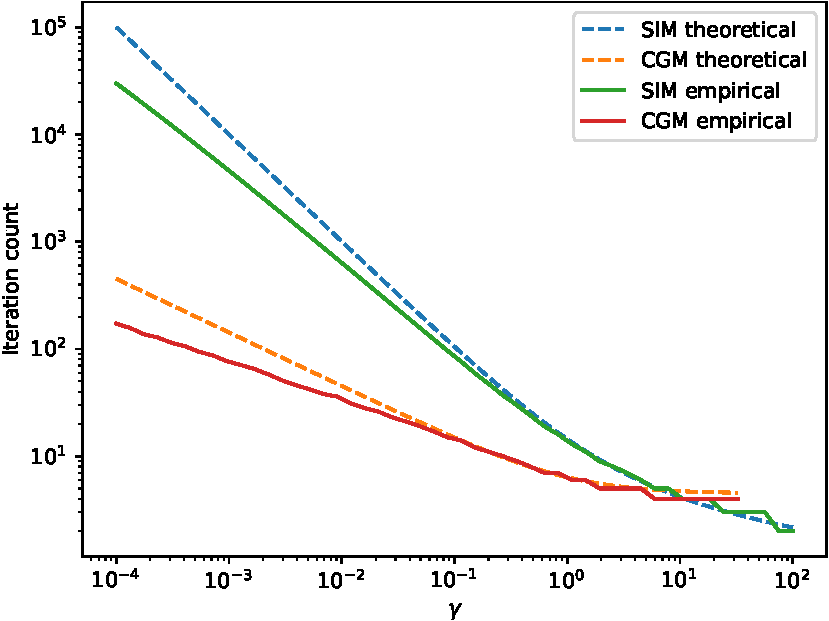
\includegraphics[width=0.7\linewidth]{Figures/gamma_plot_2d.pdf}
    \end{center}
    \caption{\small{The number of iterations required for convergence in the weak filter limit for the SIM and CGM both theoretically and empirically, as a function of $\gamma$.}}
    \label{fig:gamma_2d_plot}
\end{figure}


For the second part of experiment 1, we set $\beta = \infty$, corresponding to the strong filter limit. In this case, we expect the number of iterations to be a function of both $m$ and $\gamma$ as specified in \cref{tab:conv_SIM_CGM}. Therefore, we varied $\gamma$ in 50 logarithmically spaced increments from $10^{-6}$ to $10^2$ and $m$ in 50 linearly spaced increments from 0.01 to 0.99. For each unique pair of $m$ and $\gamma$, we then counted the number of iterations required for convergence and compared this to the theoretical predictions. The results are shown in \cref{fig:m_gamma_3d_plot}. Again, the empirical results broadly follow the theoretical functions which, as before, are scaled to fit the data. As with the weak filter limit, we again see that the empirical scaling rate is slightly better than the worst-case theoretical prediction. 

\begin{figure}[t]
    \begin{center} 
    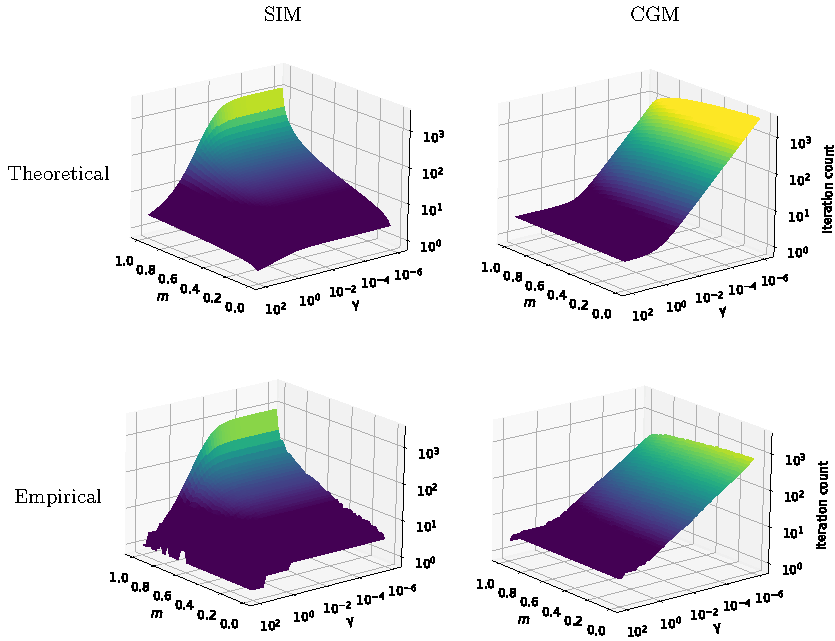
\includegraphics[width=\linewidth]{Figures/m_gamma_3d_plot.pdf}
    \end{center}
    \caption[Strog Filter Limit convergence experiments]{\small{The number of iterations required for convergence is shown both theoretically and empirically for the SIM and CGM in the strong filter limit, where $\beta=\infty$. In this case, each plot is a function of both $m$ and $\gamma$. The colourmap corresponds to vertical height and is normalised across each plot to aid comparison. }}
    \label{fig:m_gamma_3d_plot}
\end{figure}


\subsubsection{Experiment 2: Testing intermediate values of \texorpdfstring{$\beta$}{beta}}


In the second experiment, we test the number of iterations required for convergence for intermediate values of $\beta$. Note that the analysis carried out in \cref{sec:convergence} applies only for extremal values of $\beta$, meaning the intermediate behaviour is not clearly defined, and will depend on the filter chosen in practice. This was carried out for three values of $m$: 0.05, 0.5 and 0.95, representing low, medium and high prevalence of missing data respectively. For each value of $m$, we compute the solution using both algorithms over a grid of 50 $\beta$ values and 50 $\gamma$ values which were logarithmically spaced between $10^{-1}$-$10^2$ and $10^{-4}$-$10^1$ respectively. The results are shown in \cref{fig:3d_iteration_plots}. 


\begin{figure}[t]
    \begin{center} 
    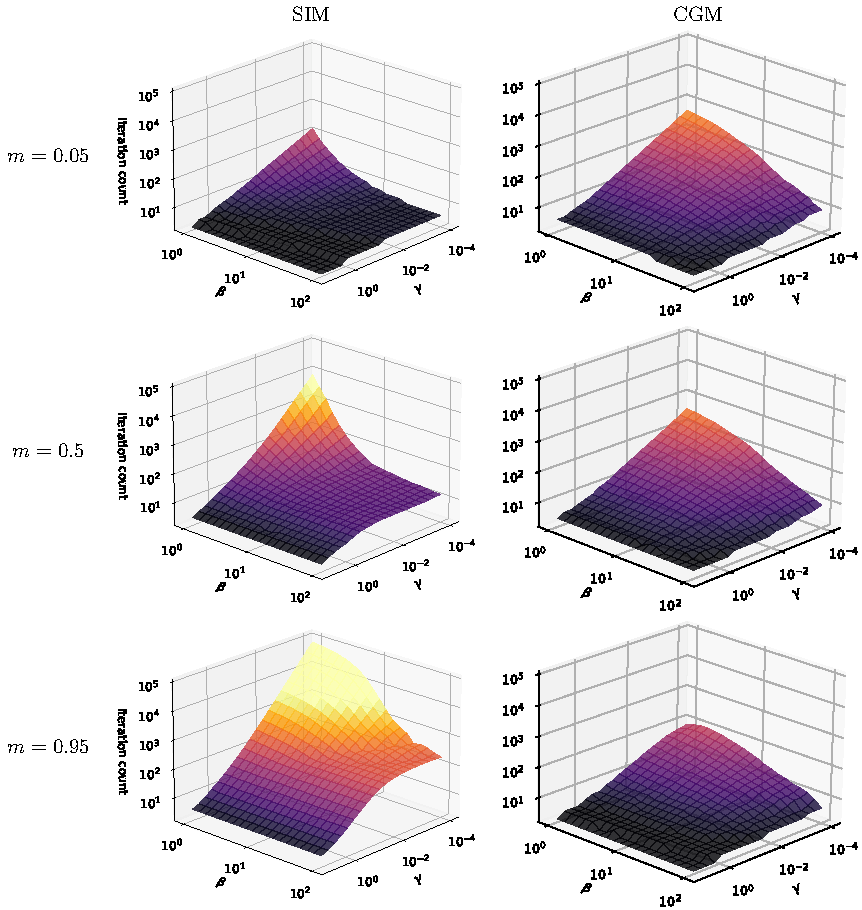
\includegraphics[width=\linewidth]{Figures/3d_iterations.pdf}
    \end{center}
    \caption[Convergence experiments]{\small{Six 3D surfaces are shown representing the number of iterations required for convergence for three values of $m$ for both the SIM and CGM algorithms. In each plot, the $x$-axis represents the filter parameter $\beta$, and the $y$-axis represents the regularisation parameter $\gamma$. The colourmap, which is normalised equally across all plots, tracks the vertical height. }}
    \label{fig:3d_iteration_plots}
\end{figure}

This experiment validates several key aspects of the theoretical convergence analysis. Firstly, notice that the basic behaviour that the number of iterations rises in all cases as $\beta$ and $\gamma$ get closer to zero. Furthermore, in all cases, regardless of the value of $m$ or $\beta$, convergence is very fast when $\gamma$ is large. We also observe the predicted behaviour that the number of iterations plateaus as a function of decreasing $\gamma$ when $\beta$ is large for the SIM while it continues to increase for the CGM. However, for this data, the CGM level seems to remain below that of the SIM in this limit. 

One key result of this experiment that aligns with the theoretical prediction is that convergence is accelerated as $m$ rises for the CGM but convergence slows as $m$ rises for the SIM. In particular, for this dataset, $n_\text{SIM} \leq n_\text{CGM}$ for all values of $\gamma$ and $\beta$ when $m=0.05$, but $n_\text{CGM} \leq n_\text{SIMM}$ for all values of $\gamma$ and $\beta$ when $m=0.95$. This is particularly impactful as it strongly indicates the CGM should be preferable when data is sparsely observed and the SIM should be preferable when the data is densely observed. 


\section{Conclusions}

The first key output of this chapter is a novel Bayesian model for the reconstruction of signals defined over the nodes of a Cartesian product graph. By introducing the concept of general anisotropic two-dimensional graph filters, we show that the posterior mean of the smooth underlying signal, $\F \in \R^{N \times T}$, is obtained by solving a linear system of size $NT \times NT$, given in \cref{eq:lin_system}. While a naive approach to computing this would have a time complexity of $O(N^3T^3)$, we propose two alternative algorithms, customised for the context of graph signal reconstruction, to compute a solution iteratively. When used in conjunction with the properties of the Kronecker product, the linear system can be solved with complexity $O(N^2T + NT^2)$ per iterative step. Furthermore, we show that this can be reduced to $O(N^2T + NT \log T)$ when considering time-vertex problems, and to $O(NT \log NT)$ when operating on a grid by making use of the Fast Cosine Transform (FCT). We demonstrated the utility of this model on a dataset comprising daily measurements of SARS-CoV-19 across local districts in the UK from February 2020 to March 2023. Our GSR model had the flexibility to reconstruct missing data in every scenario, outperforming linear interpolation and longitudinal averaging when strings of dates were removed at each district, or entire districts were removed. 

The second output of this chapter is a thorough analysis of the two iterative algorithms for obtaining the posterior mean, namely the Stationary Iterative Method (SIM) and the Conjugate Gradient Method (CGM). We show how the SIM can be implemented in an eigendecomposition free and/or distributed manner, which is of particular utility when the graph Laplacians comprising the product are large and sparse, in which case the cost per iterative step is $O\big(NT(|\mathcal{E_T}| + |\mathcal{E}_N|)\big)$. On the other hand, while both algorithms experience slower convergence when the regularisation parameter $\gamma$ is small, the CGM has superior asymptotic performance as $\gamma \rightarrow 0$, with the number of iterations scaling as $\gamma^{-1/2}$ as compared to $\gamma^{-1}$. Another interesting aspect of these two algorithms is that they have opposite behaviour in response to changes in the fraction of data, $m$, that is missing from the original graph signal. In particular, the CGM performs better when there is a high proportion of missingness, whereas the SIM performs better when there is low missingness. The precise convergence behaviour in terms of the hyperparameters $\beta$, $\gamma$ and $m$ is summarised in \cref{tab:conv_SIM_CGM}. 





